%% abtex2-modelo-trabalho-academico.tex, v<VERSION> laurocesar
%% Copyright 2012-<COPYRIGHT_YEAR> by abnTeX2 group at http://www.abntex.net.br/
%%
%% This work may be distributed and/or modified under the
%% conditions of the LaTeX Project Public License, either version 1.3
%% of this license or (at your option) any later version.
%% The latest version of this license is in
%%   http://www.latex-project.org/lppl.txt
%% and version 1.3 or later is part of all distributions of LaTeX
%% version 2005/12/01 or later.
%%
%% This work has the LPPL maintenance status `maintained'.
%%
%% The Current Maintainer of this work is the abnTeX2 team, led
%% by Lauro César Araujo. Further information are available on
%% http://www.abntex.net.br/
%%
%% This work consists of the files abntex2-modelo-trabalho-academico.tex,
%% abntex2-modelo-include-comandos and abntex2-modelo-references.bib
%%

% ------------------------------------------------------------------------
% ------------------------------------------------------------------------
% abnTeX2: Modelo de Trabalho Academico (tese de doutorado, dissertacao de
% mestrado e trabalhos monograficos em geral) em conformidade com
% ABNT NBR 14724:2011: Informacao e documentacao - Trabalhos academicos -
% Apresentacao
% ------------------------------------------------------------------------
% ------------------------------------------------------------------------

\documentclass[
	% -- opções da classe memoir --
	12pt,				% tamanho da fonte
	openright,			% capítulos começam em pág ímpar (insere página vazia caso preciso)
	twoside,			% para impressão em recto e verso. Oposto a oneside
	a4paper,			% tamanho do papel.
	% -- opções da classe abntex2 --
	%chapter=TITLE,		% títulos de capítulos convertidos em letras maiúsculas
	%section=TITLE,		% títulos de seções convertidos em letras maiúsculas
	%subsection=TITLE,	% títulos de subseções convertidos em letras maiúsculas
	%subsubsection=TITLE,% títulos de subsubseções convertidos em letras maiúsculas
	% -- opções do pacote babel --
	english,			% idioma adicional para hifenização
	french,				% idioma adicional para hifenização
	spanish,			% idioma adicional para hifenização
	brazil				% o último idioma é o principal do documento
	]{abntex2}

% ---
% Pacotes básicos
% ---
\usepackage{lmodern}			% Usa a fonte Latin Modern
\usepackage[utf8]{inputenc}		% Codificacao do documento (conversão automática dos acentos)
\usepackage[T1]{fontenc}		% Selecao de codigos de fonte.
\usepackage{lastpage}			% Usado pela Ficha catalográfica
\usepackage{indentfirst}		% Indenta o primeiro parágrafo de cada seção.
\usepackage{color}				% Controle das cores
\usepackage{graphicx}			% Inclusão de gráficos
\usepackage{float}				% Habilitar opção H nos elementos
\usepackage{microtype} 			% para melhorias de justificação
\usepackage{tikz}					% Desenho de gráficos
\usepackage{multirow}			% Trabalhando com tabelas
\usepackage{varioref}			% Inclui o comando vref

\usetikzlibrary{arrows,positioning} 
% ---
% Adicionado por Madson Dias
% ---

\usepackage{utils/termos}						% Pacote com termos comumente utilizados
\usepackage{utils/ifce-modelo} 					% Pacote com informações da customização
\usepackage{utils/ifce-facilitadores} 					% Pacote com facilitadore 
\graphicspath{ {figuras/graficos/} {figuras/imagens/}}  % Inclusão dos paths para imagens
\usepackage{xstring} 									% Criar comandos com IF
\usepackage{caption}
\usepackage{subcaption}
%\usepackage[portuguese, ruled, linesnumbered]{utils/algorithm2e}
\usepackage{amsmath}
\usepackage{amssymb}
\usepackage{colortbl}
\usepackage{listings}			% Inclusão de códigos
\usepackage{minted}				% Inclusão de códigos
\usepackage{pdfpages}
% Adiciona numeração de linhas
\lstset
{ %Formatting for code in appendix
    numbers=left,
    stepnumber=1,
}

% Altera o nome padrão do rótulo usado no comando \autoref{}
\renewcommand{\lstlistingname}{Código}

% Altera o rótulo a ser usando no elemento pré-textual "Lista de código"
\renewcommand{\lstlistlistingname}{Lista de códigos}
\renewcommand\listoflistingscaption{Lista de códigos}


% Configura a ``Lista de Códigos'' conforme as regras da ABNT (para abnTeX2)
\begingroup\makeatletter
\let\newcounter\@gobble\let\setcounter\@gobbletwo
  \globaldefs\@ne \let\c@loldepth\@ne
  \newlistof{listings}{lol}{\lstlistlistingname}
  \newlistentry{lstlisting}{lol}{0}
\endgroup

\renewcommand{\cftlstlistingaftersnum}{\hfill--\hfill}

\let\oldlstlistoflistings\lstlistoflistings
\renewcommand{\lstlistoflistings}{%
   \begingroup%
   \let\oldnumberline\numberline%
   \renewcommand{\numberline}{\lstlistingname\space\oldnumberline}%
   \oldlstlistoflistings%
   \endgroup}
\definecolor{myorange}{RGB}{230,97,1}
\definecolor{mylightorange}{RGB}{253,184,99}
\definecolor{mypurple}{RGB}{94,60,153}
\definecolor{mylightpurple}{RGB}{178,171,210}
\definecolor{mycolor1}{RGB}{35,139,69}
\definecolor{mycolor2}{RGB}{102,194,164}
\definecolor{mycolor3}{RGB}{178,226,226}
\definecolor{mycolor4}{RGB}{237,248,251}
\setlist[itemize]{noitemsep, topsep=0pt, leftmargin=1.75cm}

% ---
% Pacotes adicionais, usados apenas no âmbito do Modelo Canônico do abnteX2
% ---
\usepackage{lipsum}				% para geração de dummy text
% ---

% ---
% Pacotes de citações
% ---
\usepackage[brazilian,hyperpageref]{backref}	 % Paginas com as citações na bibl
\usepackage[alf]{abntex2cite}	% Citações padrão ABNT

% ---
% CONFIGURAÇÕES DE PACOTES
% ---

% ---
% Configurações do pacote backref
% Usado sem a opção hyperpageref de backref
\renewcommand{\backrefpagesname}{Citado na(s) página(s):~}
% Texto padrão antes do número das páginas
\renewcommand{\backref}{}
% Define os textos da citação
\renewcommand*{\backrefalt}[4]{
	\ifcase #1 %
		Nenhuma citação no texto.%
	\or
		Citado na página #2.%
	\else
		Citado #1 vezes nas páginas #2.%
	\fi}%
% ---

% ---
% Informações de dados para CAPA e FOLHA DE ROSTO
% ---
% Informações do Autor e do trabalho
% ------------------------------------
\autor{Vitor de Carvalho Melo Lopes}
\titulo{<Título da Dissertação>}
\linha{Computação aplicada} % Inteligência Artificial, Computação aplicada ou Engenharia de Software

\orientador{<Nome do Orientador>}
\coorientador{<Nome do Coorientador>} % Se você tem um coorientador, descomente esta linha

% Professores convidados para a banca
% ------------------------------------
% 
%  - Caso tenha um terceiro professor convidado, remova os comentários

\nomeprofessorA{<Nome do Professor A>}
\instituicaoprofessorA{<Instituição do Professor A> (<Sigla A>)}

\nomeprofessorB{<Nome do Professor B>}
\instituicaoprofessorB{<Instituição do Professor B> (<Sigla B>)}

%\nomeprofessorC{<Nome do Professor C>}
%\instituicaoprofessorC{<Instituição do Professor C> (<Sigla C>)}

% ---


% ---
% Configurações de aparência do PDF final

% alterando o aspecto da cor azul
\definecolor{blue}{RGB}{0,0,0}

% informações do PDF
\makeatletter
\hypersetup{
     	%pagebackref=true,
		pdftitle={\@title},
		pdfauthor={\@author},
    	pdfsubject={\imprimirpreambulo},
	    pdfcreator={LaTeX with abnTeX2},
		pdfkeywords={abnt}{latex}{abntex}{abntex2}{trabalho acadêmico},
		colorlinks=true,       		% false: boxed links; true: colored links
    	linkcolor=blue,          	% color of internal links
    	citecolor=blue,        		% color of links to bibliography
    	filecolor=magenta,      		% color of file links
		urlcolor=blue,
		bookmarksdepth=4
}
\makeatother
% ---

% ---
% Espaçamentos entre linhas e parágrafos
% ---

% O tamanho do parágrafo é dado por:
\setlength{\parindent}{1.3cm}

% Controle do espaçamento entre um parágrafo e outro:
\setlength{\parskip}{0.2cm}  % tente também \onelineskip

% ---
% compila o indice
% ---
\makeindex
% ---

% ----
% Início do documento
% ----
\begin{document}

% Seleciona o idioma do documento (conforme pacotes do babel)
%\selectlanguage{english}
\selectlanguage{brazil}

% Retira espaço extra obsoleto entre as frases.
\frenchspacing

% ----------------------------------------------------------
% ELEMENTOS PRÉ-TEXTUAIS
% ----------------------------------------------------------
% \pretextual
\imprimircapa % Capa *
\imprimirfolhaderosto % Folha de rosto *

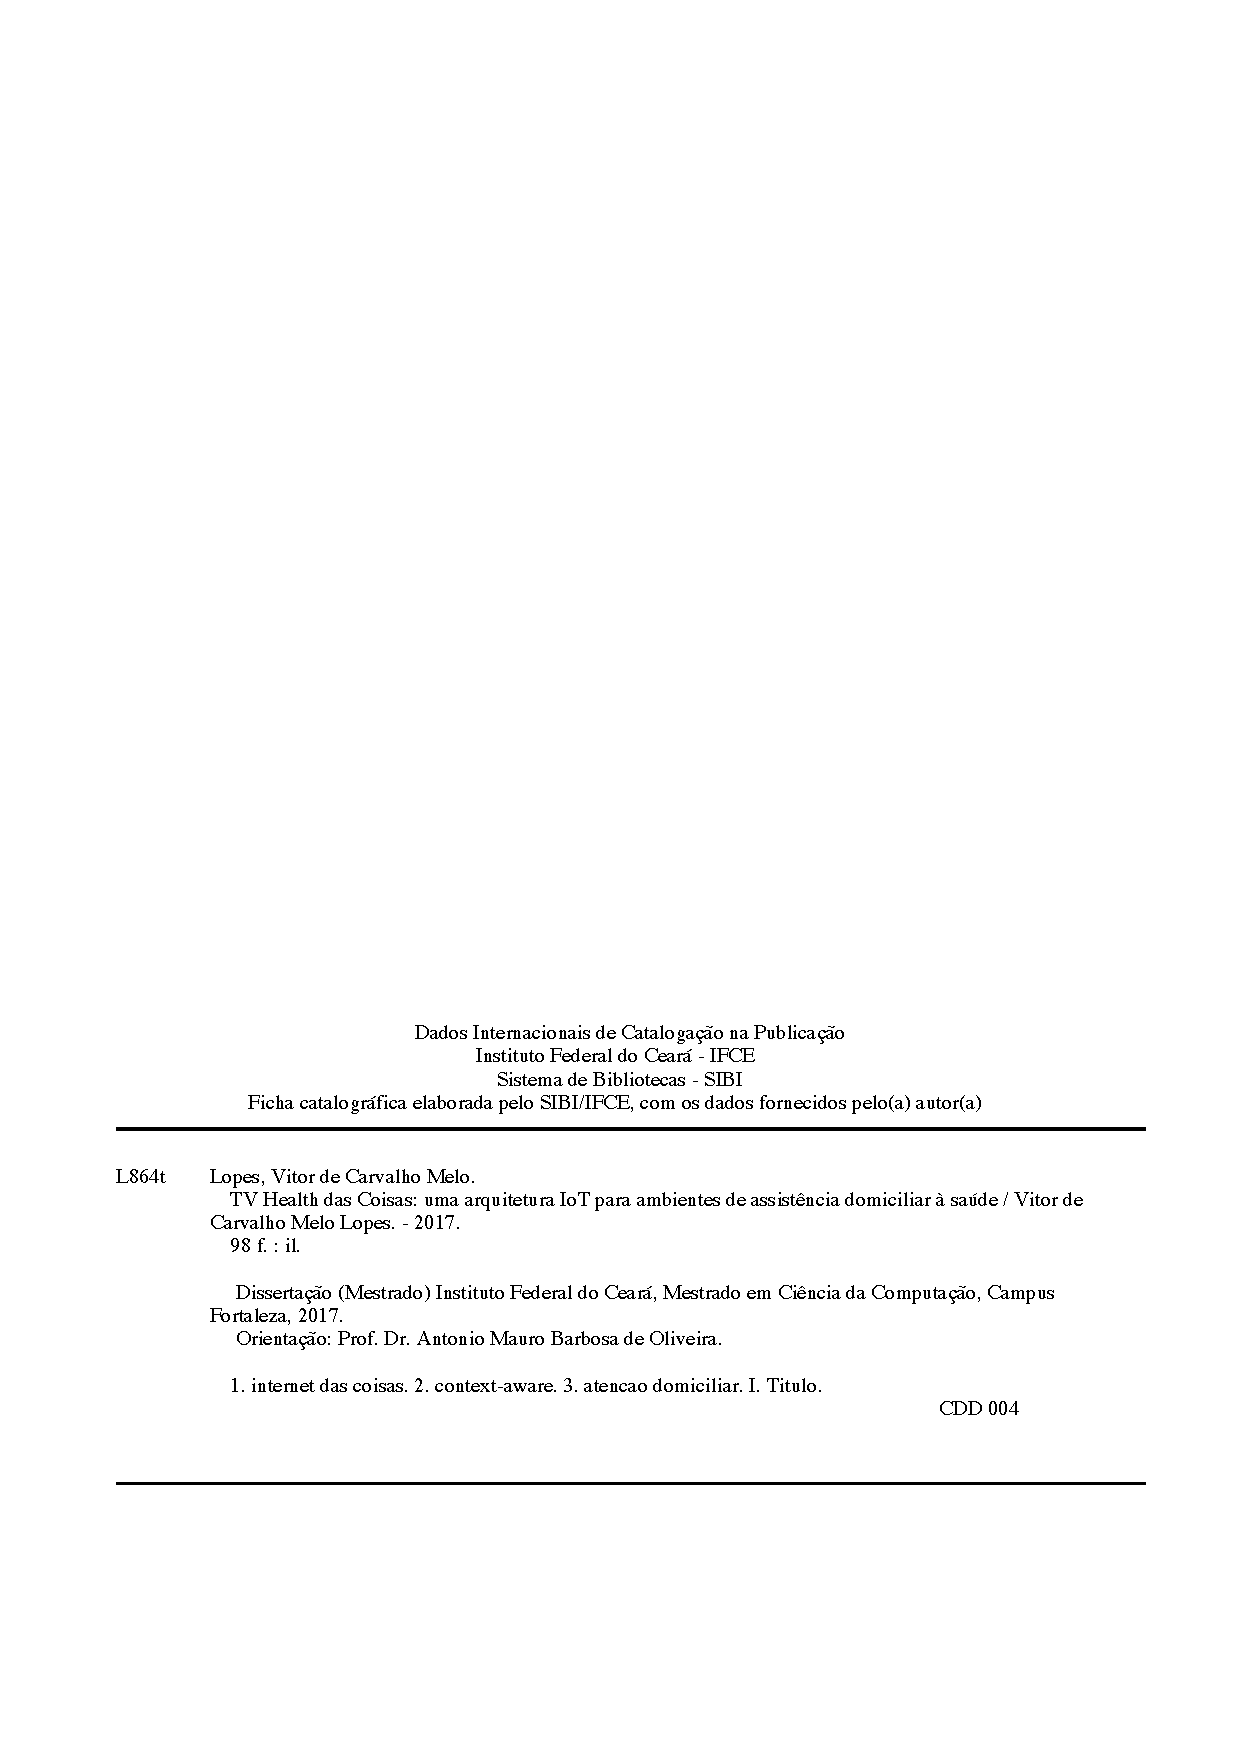
\includepdf{pretextual/ficha_catalografica}

\includepdf{pretextual/blank}
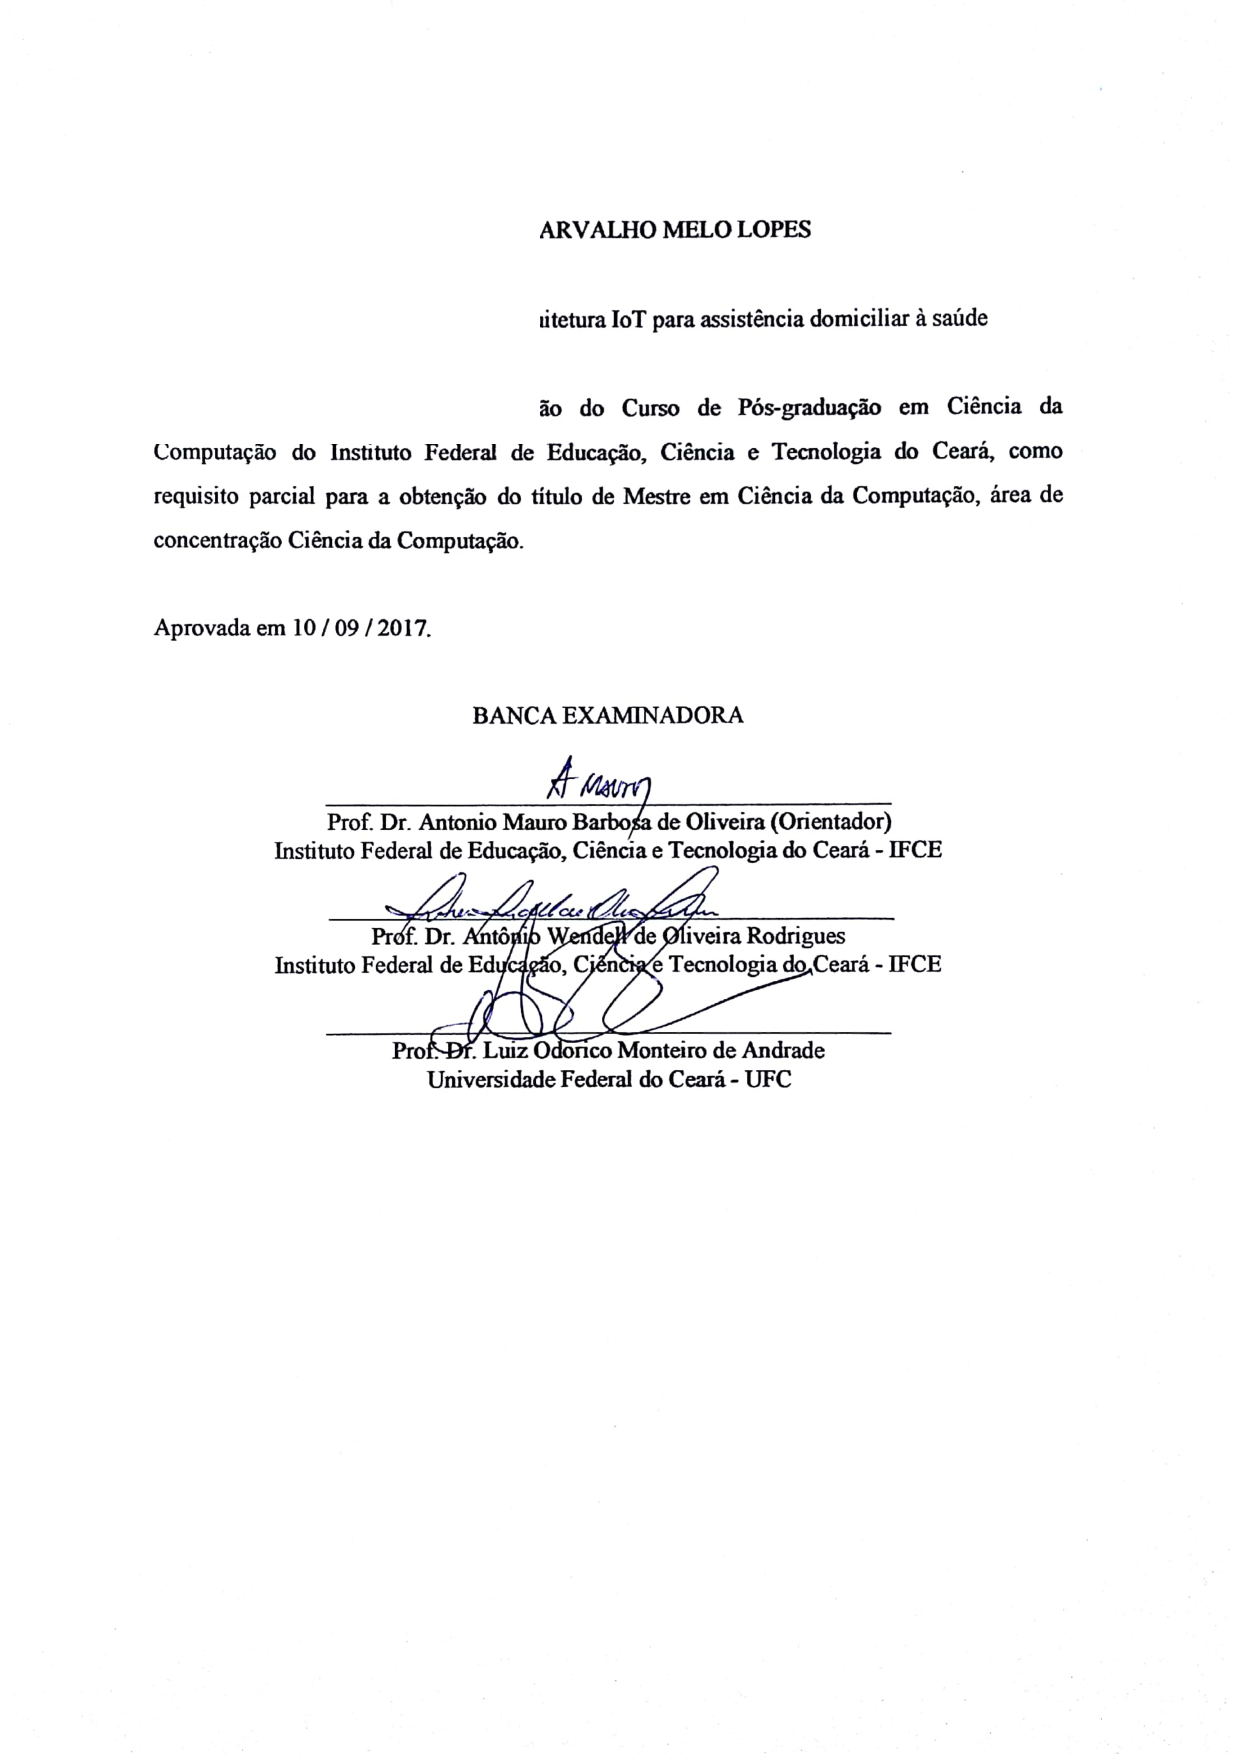
\includepdf{pretextual/folha_aceite}

\includepdf{pretextual/blank}


%\includepdf{pretextual/folhadeaprovacao.pdf} 	% Folha de aprovação (Depois da apresentação)
%\begin{dedicatoria}
   \vspace*{\fill}
   \centering
   \noindent
   \textit{ Este trabalho é dedicado às crianças adultas que,\\
   quando pequenas, sonharam em se tornar cientistas.} \vspace*{\fill}
\end{dedicatoria} 				% Dedicatória
\begin{agradecimentos}

  Aos meus pais Roberval e Ângela e irmãos Júlia e Matheus pelas alegrias compartilhadas.

  À Sofia pelo companheirismo e presença sempre carinhosa e atenciosa.

  Ao meu orientador Antonio Mauro pelos ensinamentos ao longo deste período. 

  Aos colegas de mestrado Madson, David, Renan, Gustavo e Marcelo com os quais compartilhei
  conhecimentos diversos, alegrias e dificuldades vivenciadas no laboratório LAMP/PPGCC.

  Aos colegas do Laboratório de Redes (LAR) no Instituto Federal do Ceará - Campus Aracati
  que me ajudaram com debates e ideias.

  À todos os professores do mestrado pelos ensinamentos e pelos ricos debates. 

\end{agradecimentos}
 			% Agradecimento
\begin{epigrafe}
    \vspace*{\fill}
	\begin{flushright}
		\textit{%
		``Se a preocupação está em ter, ter, ter uma pessoa cada vez se preocupará
    menos em ser, ser, ser.''\\
		(José Saramago)}
	\end{flushright}
\end{epigrafe}
 				% Epígrafe
\setlength{\absparsep}{18pt} % ajusta o espaçamento dos parágrafos do resumo
\begin{resumo}

A expectativa de vida do brasileiro aumentou de 45,5 para 75,5 anos entre 1940
e 2015, segundo dados do IBGE. Idosos podem necessitar de maiores cuidados
hospitalares com maior tempo de recuperação, o que aumenta o gasto com saúde.
Nesse sentido, a Assistência Domiciliar à Saúde (ADS) - uma modalidade de
atenção ao paciente realizado em seu próprio domicílio, – apresenta-se como
opção mais adequada ao paciente. Além de reduzir gastos hospitalares a ADS
permite o contato mais intenso com familiares na recuperação do paciente.
Estudos realizados por profissionais de saude identificaram problemas no
cenario de ADS, tais como a dificuldade que possuem os diversos atores
envolvidos: o paciente, o cuidador, familiares, equipe de saude e gestores. O
cuidador mereceu especial atenção tendo em vista que ele nem sempre possui os
conhecimentos e as habilidades necessárias para atendendimento do doente. Este
trabalho descreve a visão computacional desses cenários de saúde e propõe a TV
Health das Coisas, uma solução inteligente para o ambiente de ADS baseada no
modelo brasileiro de TV digital e na tecnologia Internet das Coisas. Esta
solução tem como substrato um sistema embarcado associado à uma TV digital
(\textit{hub}) que coleta dados de diversos sensores existentes no ambiente de ADS, além
de servir como interface para o paciente a diversas aplicações interativas. Os
dados coletados alimentam modelos inteligentes de ontologia que permitem a
inferência local (\textit{hub}) de informações necessárias à tomada de decisão dos
atores do ADS: paciente, cuidador, equipe de saúde, familiares, etc. Outro
aspecto inteligente do TV Health das Coisas diz respeito a aprendizagem de
máquinas via o sistema \nextsaude, do qual a TV Health das Coisas é um
componente. Foi definida para este cenário de ADS uma arquitetura orientada a
contexto (\textit{context-aware concept}), enriquecida com conceitos da
plataforma \textit{OpenIoT} (Plataforma de Internet das Coisas).  Um protótipo
já se encontra operacional com suas arquiteturas funcional e de engenharia
formalmente especificadas.  Assim, paciente, cuidador, familiares, equipes de
saúde e gestores podem, de forma seletiva, receber alertas, informações etc, via
TV dispositivos móveis e outros mecanismos integrados ao sistema. A TV Health
das Coisas resultou em um projeto financiado pela Embrapii e está sendo
negociado para implantação em um plano de saúde.

 \textbf{Palavras-chave}: atenção domiciliar. internet das coisas. computação ubíqua. computação pervasiva.
 \end{resumo}
 					% Resumo em português
\begin{resumo}[Abstract]
 \begin{otherlanguage*}{english}

According to IBGE, the life expectation of Brazillian people increased from
45,5 to 75,5 years between 1940 and 2015. Because of inherent fragility
of age, the elderly demands more hospital care, with more recovery time
which increases the money that the Estate spend in each patient. The
Home Care - health care modality that treats the patient in his own
home - presents as more adequate option for the patient, besides the
reduction of hospital expenses. One of the problems identified in the
scenario of home care it's the need to help the patient and the caregiver,
once that the caregiver not always have necessary knowlegde to attend
the patient. His does not always have the caregiver figure daily or in
some situations, the caregiver doesn't exist. The Information Technology
can provide mechanisms and instruments for this type of service.
Considering that the television is an equipment present in practically all
Brazillian residences, this work proposes TV Health of Things, a smart
solution for the ADS environment based on the Brazilian model of digital TV
and technology Internet of Things. TV Health of Things is a ``Set-Top Box''
(digital converter) system that collects data from various sensors in the
home care environment and serves as an interface to a variety of interactive
applications. These collected data feed ontology models that allow the
inference of information necessary for the decision making of the ADS actors
(patient, caregiver, health team, family, etc). Therefore, the various actors
mentioned can receive alerts, information, etc. via TV, web applications or 
mobile devices integrated into the system. The proposal is a component of 
\nextsaude[], a health interoperability platform based on the OpenEHR
standard. It makes use of archetypes to integrate with the \nextsaude[] platform
and thus to share services available by the platform (regulation, pharmacy
etc). TV Health of Things is a context-aware (\textit{context-aware concept}) 
architecture, enriched with concepts from the \textit {OpenIoT} platform. 
A prototype is already operational and its IoT version has its formally 
specified functional and engineering architectures.


\textbf{Keywords}: home care. iot. ubiquitous and pervasive computing.
 \end{otherlanguage*}
\end{resumo}
 				% Resumo em inglês
% inserir lista de ilustrações
\pdfbookmark[0]{\listfigurename}{lof}
\listoffigures*
\cleardoublepage
% inserir lista de tabelas
\pdfbookmark[0]{\listtablename}{lot}
\listoftables*
\cleardoublepage
% ---
% inserir lista de algoritmos
%\pdfbookmark[0]{\listalgorithmname}{loa}
%\listofalgorithms
%\cleardoublepage
% ---
% inserir lista de códigos
\pdfbookmark[0]{\lstlistlistingname}{lol}
\listoflistings
\cleardoublepage
% ---

\begin{siglas}
  \item[ABS] Anti-lock Breaking System
  \item[ADS] Assistência Domiciliar à Saúde 
  \item[SAMDU] Serviço de Assistência Médica Domiciliar e de Urgência 
  \item[SUS] Sistema Único de Saúde 
  \item[SUDS] Sistema Único e Descentralizado de Saúde 
  \item[STB] Set-Top Box
\end{siglas}  			% Lista de abreviaturas e siglas
%\begin{simbolos}
\item[$ \Gamma $] Letra grega Gama
\item[$ \Lambda $] Lambda
\item[$ \zeta $] Letra grega minúscula zeta
\item[$ \in $] Pertence
\end{simbolos} 				% Lista de símbolos
% inserir o sumario
\pdfbookmark[0]{\contentsname}{toc}
\tableofcontents*
\cleardoublepage
% ---



% ----------------------------------------------------------
% ELEMENTOS TEXTUAIS
% ----------------------------------------------------------
\textual

\chapter{Introdução}\label{cap:introducao}

O Brasil vem passando por um processo de envelhecimento da população e
um aumento da expectativa de vida crescente desde a década de 1960. 
Com os atuais índices, a taxa do envelhecimento populacional atingirá, 
em 2025, cerca de 15\% da população brasileira com indivíduos acima 
de 60 anos. 

Os mais idosos, por conta da fragilidade inerente à idade, necessitam de 
cuidados especiais na hospitalização, além de demandarem mais tempo na 
recuperação. Muitas vezes há uma demanda de vários profissionais de uma equipe 
médica multidisciplinar para se recuperar totalmente.

Essa situação afeta políticas públicas dos governos municipais, estaduais e federal -
que, segundo a Constituição Federal, deve prover atendimento hospitalar
universal à população - tornando o gasto público com hospitalização de idosos
maiores a cada ano.

Portanto, esse processo que a população brasileira vem sofrendo, ocasiona mudanças 
nos paradigmas de atendimento à saúde. Nessa perspectiva, surge a atenção domiciliar
%Uma outra abordagem para casos semelhantes é a atenção domiciliar
ou \textit{home care}, modelo definido como o tratamento do paciente 
em seu próprio lar, com a presença ou não de um cuidador - figura responsável
por acompanhar o idoso em suas atividades diárias, ao assumir um papel 
de fundamental importância no acompanhamento do paciente em seu cotidiano. 

Pesquisas mostram que esse método traz benefícios pois o 
paciente encontra-se em um ambiente conhecido e está na presença contínua de
seus familiares.

Assim, pesquisas realizadas indicam uma mudança gradativa no modelo de
tratamento de idosos. A escolha da atenção domiciliar em detrimento da
hospitalização traz benefícios sociais, psicológicos e
econômicos para o paciente. %, mas também benefícios econômicos para o Estado.

No que concerne às políticas públicas desenvolvidas pelo Estado, 
a vantagem é de reduzir os custos com internação. Estudos revelam 
que é possível reduzir custos de internação hospitalar com uma 
abordagem em atenção domiciliar nos casos de menor gravidade, 
ou seja, casos em que o paciente não corre risco de morte. 
% o aumento de casos em que o paciente pode ser tratado v

\section{Motivação para a Dissertação}\label{sec:motivacao}

Observo na sociedade atual, através de notícias divulgadas, nos meios
de comunicação, de conversas informais, de filmes etc que está cada
vez mais crescente a preocupação com os idosos, haja vista o
aumento da expectativa de vida. Me pergunto como é possível essas pessoas
terem uma qualidade de vida na velhice se sabemos que, nessa idade,
os problemas de saúde são acentuados, como falta de autonomia,
dificuldades de locomoção, preocupação com remédios etc.

Em muitos casos, cresce o número de internações hospitalares e,
consequentemente, os gastos do Estado. Visando enfrentar essa 
realidade, a comunidade acadêmica, % a partir de meados dos anos tais,
começa a se pesquisar sobre os cuidados aos idosos no espaço domiciliar.

A linha de pesquisa de computação aplicada à saúde é vista como uma parte
importante para a melhoria na qualidade dos serviços prestados na área.
Com a pesquisa realizada, a comunidade acadêmica possibilitou o avanço
de atenção domiciliar, pesquisando e desenvolvendo sistemas inteligentes
que auxiliem no tratamento e ajudem os envolvidos.

\section{Descrição do problema}\label{sec:descricao-problema}



A partir do descrito, se pode identificar que a internação domiciliar
de pacientes idosos é possível. O auxílio ao idoso, ao cuidador
ou ainda, à equipe médica que o acompanha carece de soluções eficientes
e acessíveis financeiramente.

\section{Objetivos Geral e Específicos}\label{sec:objetivos}

Em seu sentido mais particular, os seguintes objetivos específicos são:

\begin{itemize}
	\item ...; 
	\item ...;
\end{itemize}

\section{Produção científica}\label{sec:producao}
Durante este projeto de mestrado, os seguintes trabalhos científicos foram aceitos e publicados, a saber:

\begin{itemize}
	\item \textbf{Einstein, A.}, 1905. \textbf{The photoelectric effect}. Ann. Phys, 17(132), p.4;
	\item \textbf{Einstein, A.}, 1904. \textbf{Zur allgemeinen molekularen Theorie der Wärme}. Annalen der Physik, 319(7), pp.354-362.
\end{itemize}

\section{Estrutura da Dissertação}\label{sec:estrutura}
\lipsum[1]
 				% Capítulo 1 - Introdução
\chapter{Fundamentação Teórica}\label{cap:fundamentacao-teorica}

Este capítulo apresenta a fundamentação teórica, separada em aspectos de saúde e
tecnológicos. As seções de saúde abordam termos como Assistência Domiciliar à
Saúde e suas particularidades, além de explanar, brevemente, sobre a história da
hospitalização no Brasil. A seção \ref{sec:aspectos-tecnologicos} trata das
tecnologias e conceitos tecnológicos utilizados neste trabalho.

\section{Aspectos de Saúde}\label{sec:aspectos-de-saude}

Segundo \citeonline{inaia2008}, uma das primeiras instituições voltadas para o
cuidado com a saúde foi a fundação da Santa Casa de Misericórdia de Santos, em
1543, cuja principal atividade era prestar assistência de cunho caritativo a
pessoas pobres e desabrigados. Tal estrutura permanece inalterada até o final do
século XIX, e início do século XX.

Com o Governo Getúlio Vargas, a partir de 1930, ocorre no Brasil o processo de
industrialização, que trouxe crescimento rápido e desordenado às cidades,
principalmente São Paulo e Rio de Janeiro. As transformações econômicas e
sociais resultantes desse processo, a falta de saneamento básico, a pobreza etc
foram motivos para que parte da população reivindicasse mais atenção do Governo
em relação aos cuidados de saúde \cite{carvalho1984}.

\citeonline{carvalho1984} indica, ainda, que apesar dessa pressão, não existiu
uma política de saúde clara por parte das autoridades. Muitas vezes, algumas
ações se voltavam para a criação de condições sanitárias mínimas, que se
mostravam limitadas frente às reais necessidades da população. Dessa forma, as
décadas subsequentes não foram significativas no tocante a uma ampliação dos
serviços de saúde oferecidos à população.

Conforme análise de \citeonline{inaia2008}, ainda nos anos 1970, surgem
tentativas de universalizar o acesso à assistência à saúde. Alguns programas e
sistemas foram iniciados, sendo válido citar, (i) Sistema Único e
Descentralizado de Saúde, o SUDS e (ii) o Sistema Único de Saúde, o SUS.
Entretanto, em virtude da vigência da ditadura militar, implantada em 1964, que
levou o país a vivenciar um estado de exceção, tais propostas não conseguiram se
concretizar. Assim, somente no período da redemocratização, ocorrida em meados
dos anos 1980, é que o SUS foi criado oficialmente pela Constituição Federal de
1988, Lei 8080/90\footnote{ Acessível em
\url{http://www.planalto.gov.br/ccivil_03/leis/L8080.htm}}, com o  objetivo de
garantir à população Brasileira, o acesso universal às ações e  serviços de
saúde.

Paralelo à criação do Sistema Único de Saúde (SUS), ocorreu o avanço
tecnológico que alcançou a prática médica, aperfeiçoando, com isso a
infraestrutura hospitalar. Dessa forma, os hospitais deixaram de ser espaços
para abrigarem pobres desamparados e passaram a proporcionar tratamentos mais
elaborados. O hospital passa a oferecer  procedimentos cirúrgicos, atendimentos
de urgência, internações, tornando a instituição complexa, com uma atuação de
caráter menos íntimo e acolhedor. Além disso, estudiosos começam a identificar
a possibilidade de tratamentos e cuidados com a  saúde que não estejam,
necessariamente, vinculados ao ambiente hospitalar.

Como consequência, surgiram diversas mudanças no atendimento, onde a Assistência
Domiciliar à Saúde (ADS) se tornou uma modalidade disponível.

\subsection{Assistência Domiciliar à Saúde}
\label{subsec:assistencia-domiciliar-a-saude}

A Assistência Domiciliar à Saúde (ADS) divide-se basicamente em grupos de
enfermagem e fisioterapia - nas modalidades mais básicas - até um atendimento
multiprofissional, possibilitando um apoio ao paciente como um todo. A ADS pode
ser provida tanto pelo setor privado quanto pelo setor público
\cite{amaral2001assistencia}.

Os primeiros registros da ADS no Brasil surgem em 1967, na cidade de São
Paulo, no Hospital do Servidor Público. O principal objetivo dessa abordagem
era a liberação de leitos no hospital, levando para o domicílio procedimentos
básicos, de baixa complexidade clínica.

No começo da década de 90, segundo \citeonline{tavolari2000desenvolvimento},
houve um aumento na quantidade de empresas privadas provendo o serviço de ADS,
com atuação de cinco empresas que prestavam esse tipo de  serviço. Já em 1999,
esse número subiu, consideravelmente; para mais de 180
\cite{tavolari2000desenvolvimento}.

\citeonline{amaral2001assistencia} define a ADS como uma sequência de serviços
residuais a serem oferecidos, depois que o indivíduo já recebeu atendimento
primário e prévios, ou seja, aquele que já recebeu atendimento primário com
consequente diagnóstico e tratamento.

\citeonline{amaral2001assistencia} lembram, ainda, que o atendimento domiciliar
pode acelerar a recuperação do  paciente e promover a redução de custos
hospitalares, além de ser uma solução mais  humanista para os portadores de
doenças crônicas ou de longa duração, frente à  hospitalização. Dessa forma, a
assistência domiciliar à saúde tem como objetivos principais: (1) humanização
no atendimento; (2) maior rapidez na recuperação do paciente, devido à
proximidade com os seus familiares; (3) diminuição do risco de infecção
hospitalar; (4) Otimização de leitos hospitalares para pacientes que deles
necessitem; e (5) Redução do custo/dia da internação.

\subsubsection{Envolvidos}\label{subsubsec:envolvidos}

Para o entendimento geral da modalidade ADS, faz-se necessário separar e
explicar a atuação de cada um dos envolvidos. O paciente, para quem está
voltado, fundamentalmente, todo o sistema, é aquele que sofre algum problema
físico ou mental. A família é responsável por prover um ambiente propício à
melhora do paciente.

Outra figura importante na atenção ao paciente é a equipe multiprofissional -
composta de médicos, enfermeiros, psicólogos, terapeutas, assistentes sociais,
farmacêuticos, cuidadores e outros - visando propiciar, através da integração
das diversas áreas de conhecimentos, a melhoria efetiva do paciente.

O cuidador, muitas vezes, é um familiar, alguém próximo à família ou alguém
contratado. Seu papel principal é cuidar do paciente, ajudando nas tarefas
diárias, como alimentação, lazer, socialização, limpeza do paciente, entre
outros \cite{amaral2001assistencia}.

%Embora as pesquisas indiquem que o tratamento domiciliar ajuda na recuperação do
%paciente, devido sua presença no seio familiar, também sabemos das dificuldades
%que os cuidadores enfrentam. exemplo quando são familiares, que muitas vezes, 
%negam a dar atenção, ou desempenhar determinadas funções.

\subsubsection{Terminologia}\label{subsubsec:terminologia}

Apesar de não haver uma definição formal, a Assistência Domiciliar à Saúde pode
ser separada em três modalidades, diferenciadas, principalmente, pelo grau de 
atenção dispensada ao paciente. 

É defendido por Tavolari, Fernandes e Medina, que o termo Assistência Domiciliar
à Saúde é genérico e referente a todo e qualquer procedimento de saúde realizado
em domicílio, não importando o grau de complexidade. Já o termo Internação
Domiciliar é aplicado quando, dos procedimentos realizados, o cuidado intensivo
e multiprofissional é perceptível, caracterizando-se ainda, pelo transporte de
parte da estrutura hospitalar para o domicílio do paciente. O paciente, nesse
caso, é categorizado com complexidade alta ou moderada.
Já no Atendimento Domiciliar, o paciente encontra-se num estado de menor 
complexidade médica, e a atenção a ele dispensada pode ou não ser realizada por
uma equipe multiprofissional \cite{tavolari2000desenvolvimento}.

\figuradupla{ads-tavalori}{Representação gráfica das categorias defendida 
por Tavolari, Fernandes e Medina}{ads-giacomozzi}{Representação gráfica das 
categorias defendida por Giacomozzi}

\citeonline{giacomozzi2006pratica} faz uma inversão das categorias propostas
por \citeonline{tavolari2000desenvolvimento} e  define Atenção Domiciliar à
Saúde como um termo mais genérico, englobando o atendimento, a visita e as
internações domiciliares \cite{giacomozzi2006pratica}. Segundo a autora, a
atenção domiciliar é ``um componente do \textit{continuum} dos cuidados à
saúde, pois os serviços de saúde são oferecidos ao indivíduos e sua família
[...] minimizando os efeitos das incapacidades ou doenças, incluindo aquelas
sem perspectiva de cura.'' Já o termo Assistência Domiciliar à Saúde, é formado
por atividades de cunho ambulatorial, adicionando a essa categorização a
modalidade Visita Domiciliar, voltada para verificar a realidade do paciente,
além de realizar ações educativas.

A despeito da diversidade de categorização apresentada pelos autores, ao nosso
trabalho interessa tanto aqueles pacientes que inspiram maiores cuidados,
correndo, inclusive, risco de vida, quanto aqueles que demandam menos
preocupações - mas que, invariavelmente, estão sob os cuidados fora do
ambiente hospitalar.

\section{Aspectos Tecnológicos}\label{sec:aspectos-tecnologicos}

Este trabalho foi amparado em tecnologias bem conhecidas, permitindo assim, 
que os objetivos fossem alcançados.

\subsection{Sistemas Embarcados}\label{subsec:sistemas-embarcados}

Sistemas Embarcados estão inseridos em nossos cotidianos. Aparelhos como
\smartphones[], \tablets[] - com alto poder de processamento,
produtos comumente encontrados em nossas casas, a exemplo do forno de 
micro-ondas, geladeiras e máquinas de lavar roupas, até computadores de bordo e
controle de freios ABS (\textit{Anti-lock Breaking System})\footnote{ABS:
Tecnologia  de freio considerada segura pois seu funcionamento impede que, em
uma brecada brusca, as rodas  deslizem, tornando difícil controlar o veículo} em
nossos carros, contêm sistemas embarcados. Essa diversidade de aplicações
explicita a importância dessa área.

Nos exemplos citados anteriormente, temos uma classificação quanto à sua
funcionalidade, porém, sua definição não é simples, nem muito menos taxativa,
uma vez que possuem uma grande complexidade em sua composição. Dessa forma,
podemos definir, a princípio, sistemas embarcados como qualquer
dispositivo/equipamento que disponha de um sistema programável e que seu
objetivo não seja o de um computador de propósito geral\footnote{Computador de
propósito geral é aquele em que é possível executar as mais diversas tarefas,
tais como, navegar na Internet, escrever documentos, executar jogos etc, ou
seja, não há uma função específica a ser realizada. Pelo exposto, percebe-se a
complexidade da definição de sistemas embarcados, uma vez que, muitos deles, 
desempenham funções que antes cabiam apenas ao computador de propósito geral.}
\cite{wolf2012computers}.

Marwedel define: ``Sistemas Embarcados (como) sistemas de processamento de
informações incorporados à produtos.'', e, adicionado à esta definição, lista 5
características que devem levar em consideração: 

\begin{itemize}
  \item Segurança - ou seja, os dados confidenciais transmitidos ou recebidos pelo
  equipamento devem permanecer confidenciais e a comunicação deve ser autêntica;
  \item Seguro - característica indicativa de que o sistema não causará nenhum dano àqueles que o utilizam;
  \item Disponibilidade - sistema disponível para executar as funções para as quais
  foi programado; 
  \item Confiabilidade - probabilidade que o sistema tem de que não
  falhará em sua execução; e
  \item Manutenibilidade, caso o sistema venha a falhar, deverá 
  ser consertado em uma determinada janela de tempo.
\end{itemize}

Além disso, propriedades como sensores coletando informações do ambiente
físico e atuadores controlando o ambiente no qual estão inseridos também
caracterizam um sistema embarcado \cite{marwedel2010embedded}.

\subsubsection{Arquitetura}\label{subsubsec:arquitetura}

A literatura divide o sistema embarcado em duas áreas, o \hardware[] e o 
\software. O primeiro é composto pelas partes físicas do sistema, 
tal como o processador, memória, interfaces de entrada e saída etc. O segundo é
composto pelos componentes lógicos do sistema, ou seja, os programas que 
irão executar as funções previamente definidas do sistema embarcado.

No processo de \design[] do sistema embarcado considera-se, dentro dos
requisitos de \hardware, quais dos processadores disponíveis no mercado atende
melhor a necessidade do projeto, assim como é necessário identificar a
quantidade de memória a ser utilizada pelo \software[]. 

Ainda referente ao processo de design é necessário determinar quais serão as
interfaces de entrada (responsáveis por receber os dados para posterior
processamento) e as interfaces de saída (responsáveis por apresentar os dados
processados). Em paralelo, os requisitos de \software[] são alinhados para que o
\hardware[] seja melhor aproveitado \cite{wolf2012computers}.

A depender da finalidade do produto, esses requisitos diferem bastante. Por
exemplo, o sistema embarcado responsável por controlar uma máquina de lavar é
simples (em termos de funcionalidade, processamento, consumo de energia etc),
uma vez que aplica um componente microcontrolador de baixo poder de
processamento (tal qual um microprocessador PIC de 16 bits) e um circuito
auxiliar para atender as especificações de entrada e saída do sistema, assim
como uma possível comunicação com outros sistemas.

Já o sistema embarcado em um \smartphone[] realiza diversas funções, tem um
alto nível de processamento de dados e consome muita energia. Para atender a
estes requisitos, a equipe responsável pelo \design[] utiliza vários
processadores de alto poder computacional (tal qual processadores ARM), como
interface de entrada e saída uma tela sensível ao toque e faz uso, ainda, de
diversos sensores para ajudar na usabilidade do dispositivo.

Semelhante aos \smartphones, o sistema embarcado utilizado neste trabalho, o
Set-Top Box (STB), processa grande quantidade de dados, além de realizar
diferentes funções. Em que pese tais diferenças, o \hardware[] utilizado é
bastante semelhante.

\subsection{Computação ubíqua e pervasiva}\label{subsec:computacao}

A convergência das diversas tecnologias pode ser observado no nosso dia-a-dia
através de: informações constantes que recebemos nos dispositivos móveis, nos
meios de comunicação, do monitoramento em tempo real do tráfego nas cidades de
grande porte, dos relógios com tecnologia embarcada (\textit{smartwatches}), das
vestimentas inteligentes etc.

Percebemos, também, o distanciamento ou o desaparecimento da figura ``computador
pessoal (PC)'', em nosso cotidiano. A tecnologia está difundida ao ponto do
termo  ``era pós pc'' ser encontrado em diversos estudos
\cite{bonilla2011inclusao,  chen2011pospc, press1999personal} nas áreas de
sistemas embarcados e  tecnologias móveis.

À essa tecnologia ``em todo lugar'' e ao distanciamento do usuário com o 
computador pessoal deu-se o nome de computação ubíqua. Mark Weiser, considerado 
o pai desse termo, antecipou que encontraríamos tecnologia nos diversos objetos
do nosso cotidiano, tais como etiquetas de roupas e alimentos, cadeiras, 
geladeiras, lixeiras, interruptores de luzes etc \cite{weiser1991computer}. Essa 
previsão de Weiser já se concretizou em vários dispositivos.

Através de sensores e meios de comunicação, esses objetos ganham novas funções.
A patente de Yang registra uma lixeira inteligente que abre sua tampa de acordo
com a proximidade do usuário \cite{yang2005trash}. Já a pesquisa de Wang
demonstra a utilização de sensores em uma geladeira. A partir de um sistema de
gerenciamento da geladeira é possível ter informações das comidas e recomendar
receitas para o usuário de acordo com os alimentos disponíveis, além de 
verificar quais itens estão próximos do final da validade ou faltantes e gerar 
uma lista de compras personalizada \cite{hou2013}.

% Os dispositivos \smartphones, \tablets, relógios inteligentes e até mesmo roupas
% inteligentes são realidades para muitos. Esses dispositivos permitem que o 
% indivíduo que os carrega, tenha um poder computacional que o permita utilizar 
% serviços que um computador oferece, independentemente da sua localização 
% \cite{de2003computaccao}.

Muitas vezes, a tecnologia inserida nesses objetos é invisível para o usuário
final e essa transparência era defendida por Weiser para apresentar um outro
termo, a ``computação pervasiva'', assim definida pelo autor: ``(...) criar  um
computador tão embarcado, tão natural que o usaríamos sem nem pensar sobre
ele''. Além disso, computação pervasiva está relacionada à capacidade de
dispositivos serem embarcados no mundo físico, obtendo informações do meio para
auxiliar na computação, integrando, dessa forma, o ambiente físico e o mundo
virtual \cite{bolsoni2009computaccao, de2003computaccao}. A figura  
\ref{fig:pervasive-marwedel} demonstra a interligação entre as áreas de sistemas
embarcados, computação ubíqua e pervasiva com as tecnologias de comunicação.

\figurasimples{pervasive-marwedel}{Representação gráfica das influências nas 
áreas de sistemas embarcados, computação ubíqua/pervasiva e meios de 
comunicação.}{12cm}

Segundo Hansmann, a computação pervasiva tem 4 princípios fundamentais,
detalhados a seguir \cite{hansmann2013pervasive}:

\begin{description}
  \item [Descentralização] os diversos dispositivos cooperam entre si e realizam
  pequenas tarefas e funções, contribuindo para o estabelecimento de uma 
  dinâmica rede de comunicação; Podemos citar como exemplo os diversos 
  dispositivos implantados na casa proporcionando conectividade em toda
  a extensão da casa.
  \item [Diversificação] diferente do computador de propósito geral - que 
  proporciona a execução de várias tarefas - cada dispositivo tem um propósito
  específico atendendo a necessidades únicas; podemos citar, como exemplo, um
  sensor para leitura do nível de oxigênio no sangue, um relógio inteligente
  que conta quantos passos uma pessoa deu durante o dia etc; dentro dessa 
  diversidade, cada um desempenha uma função específica.
  \item [Conectividade] os dispositivos devem interagir de maneira transparente
  e aqueles que são móveis, devem mudar entre redes heterogêneas, sem o 
  auxílio de um usuário; a conectividade diz respeito, também, à relação 
  transparente entre dispositivo e usuário; 
  \item [Simplicidade] as funções desempenhadas pelos dispositivos devem ser
  simples e de fácil execução. Existem tipos de dispositivos que não requerem 
  uma interação com o usuário; outros, no entanto, exigem alguma configuração e,
  nestes casos, a interação deve manter-se simples, capaz de oferecer acesso
  rápido ao usuário. 
\end{description}

No que concerne à assistência domiciliar à saúde, as pesquisas nas áreas de
computação ubíqua e pervasiva são as mais diversas. Isso porque o domicílio é um
ambiente propício à aplicação dessas técnicas. A utilização de sensores, como
demonstrado no estudo de Warren, em que sensores  vestíveis são empregados na
leitura de oxigênio do paciente e o envio dos dados à um sistema de
monitoramento pessoal para posterior processamento \cite{warren2002sensors}
exemplifica a utilização da computação pervasiva, uma  vez que os dados
coletados se tornam disponíveis a qualquer momento.

\subsubsection{Internet das Coisas} \label{subsubsec:iot}

No final dos anos 90, \citeonline{ashton2009internet} defendeu que a Internet
das Coisas tinha potencial para mudar o mundo, assim como a Internet mudou.
Desde então pesquisas em diversas áreas, a inovação tecnológica e a atualização
de conceitos já existentes possibilitou o surgimento da tecnologia Internet das
Coisas (\textit{Internet of Things - IoT}).

Na revisão sistemática sobre IoT, \citeonline{li2015internet}, defende IoT como
parte da Internet do futuro e consiste de bilhões de ``coisas'' inteligentes
que se comunicam entre si. Já \citeonline{pretz2013next} define IoT como um
conjunto de coisas conectadas por uma rede sem fio e que são capazes de
interagir entre si, sem interferência humana. Já
\citeonline{guillemin2009internet} define Internet of Things permite que
pessoas e coisas estejam conectadas a qualquer hora, em qualquer lugar com
qualquer coisa e qualquer um, preferencialmente usando uma rede e qualquer
serviço.

\figurasimples[perera2014context]{iot-perera}{Ilustração da definição de IoT.}{8cm}

%Apesar da capacidade de trocar dados entre si, alguns autores como, Dada e
%Thiesse, Broll e Gama et al argumentam que a falta de padrões pode diminuir a
%competitividade de produtos IoT. Por esse motivo, esses mesmos autores
%trabalham em comissões internacionais para padronizar protocolos de
%comunicação.

IoT habilita sistemas a capturar, armazenar e  transmitir dados de modo que
cresce a quantidade de áreas atendidas por esse tipo de tecnologia.
Alimentação, segurança, indústrias, logística, turismo e armazenamento são
algumas das áreas em que a aplicação de IoT é abrangente e traz benefícios
\cite{xu2014ubiquitous}.

A área de atendimento domiciliar é uma importante área de aplicação de IoT.
Segundo \citeonline{xu2014ubiquitous}, IoT é adotado para melhorar a qualidade
do serviço e reduzir custos. Um número cada vez maior de sensores médicos e
dispositivos capazes de capturar sinais vitais do paciente  - como por exemplo
temperatura corporal, nível de glicose no sangue, e pressão sanguínea - estão
surgindo, possibilitando um monitoramento do paciente em tempo real.

\subsection{Aplicações Sensíveis ao Contexto}\label{subsec:contexto}

O dicionário Houaiss define contexto como um conjunto de palavras, frases ou
texto que precede ou se segue a determinada palavra, frase ou texto e que
contribuem para o seu significado. Podemos entender desta definição que contexto
são circunstâncias que acompanham a situação ou determinado fato. A depender do
contexto, nos portamos de maneira diferente, como por exemplo: nos portamos de
uma maneira no ambiente de trabalho (contexto) e de uma maneira diferente quando
estamos na praia (contexto).

% Na comunicação entre pessoas, aproveitamos o contexto para facilitar, ou ainda,
% acelerar a velocidade da conversa, mas não é fácil a utilização de contexto nas
% comunicações homem-máquina.

Apesar de exemplificar de maneira clara o que é contexto, esse tipo de definição
apresentada anteriormente é de difícil aplicação na área da computação.
Outras abordagens com definições mais específicas foram surgindo com o
passar do tempo. No trabalho de Schilit et al são definidos 3 aspectos
importantes para o contexto, (1) onde você está, (2) com quem você está e (3)
quais recursos estão próximos \cite{schilit1994context}. Pascoe define contexto 
como um conjunto de estados de interesse conceituais e físicos para uma entidade 
em particular \cite{pascoe1998adding}.

O desenvolvedor precisa identificar se determinada informação é contexto ou não
para determinada aplicação em determinado momento. Tomando como exemplo uma
aplicação móvel de acompanhamento de um \textit{tour} em um museu a céu aberto, 
tanto as informações de tempo (clima, precipitação, umidade etc) quanto as 
informações de pessoas (quantidades em cada setor) são informações de contexto, 
já em locais fechados, a informação de tempo não representa uma informação de 
contexto.

Davies realizou um trabalho semelhante ao apresentado acima. Foi 
desenvolvido uma aplicação de guia turístico sensível a contexto para a cidade 
de \textit{Lancaster} na Inglaterra. A solução combinava computação móvel, 
comunicação sem fio e sistemas embarcados para prover aplicações interativas
\cite{davies1999caches}.

No sentido de simplificar o desenvolvimento de aplicações sensíveis ao contexto,
Dey define "contexto (como) qualquer informação que pode ser utilizada para
caracterizar a situação de uma entidade. Uma entidade pode ser uma pessoa, um
lugar ou um objeto que é considerado relevante para a interação entre um usuário
e uma aplicação, incluindo o usuário e a aplicação".

É possível, portanto, definir que um sistema computacional é sensível ao contexto
se ele fizer uso do contexto para prover informações ou serviços relevantes para
o usuário de acordo com a sua tarefa no momento \cite{dey2001understanding}.

No que concerne a assistência domiciliar à saúde, os sistemas sensíveis a
contexto podem fazer uso de informações de sensores médicos (leitura de sinais 
vitais do paciente), sensores de propósito geral (leituras no ambiente), 
ou ainda sensores virtuais (conjunto de programas cuja função é varrer as redes 
sociais e extrair informações válidas para determinada situação).

\subsection{Plataforma OpenIoT}\label{subsec:openiot}

O OpenIoT é um esforço conjunto da União Européia para Pesquisa e Inovação (FP7
- \textit{European Union's Research and Innovation}). A plataforma 
\textit{OpenIoT} tem como objetivo principal a implantação de uma infraestrutura 
de \textit{middleware} capaz de integrar soluções de Internet das Coisas.

O projeto enfatiza a convergência de Internet das Coisas e computação em nuvem,
habilitando esses dois tópicos através de interoperabilidade semântica e dados
ligados (\textit{Linked Data}), desse modo, será possível fornecer aos
interessados uma "nuvem de coisas". A figura \ref{fig:arquitetura-openiot} a 
seguir representa  as partes que compõem a plataforma OpenIoT.

\figurasimples[soldatos2015openiot]{arquitetura-openiot}{Arquitetura plataforma 
\textit{OpenIoT}}{12cm}
    
A plataforma foi arquitetada com 3 grandes seções: (1) Aplicações e Utilitários,
(2) Plano virtualizado e (3) Plano físico. Diversos componentes compõem as 
seções, listados abaixo, com uma visão \textit{top-down}:

\begin{description}
  \item [Aplicações e Utilitários]
  \item [Request Presentation] Responsável pelas apresentações das saídas dos serviços,
ou seja, permite a seleção de mashups a partir de uma biblioteca com o intuito
de facilitar a apresentação dos objetos configurados em uma interface web. Para
isso, esse módulo comunica-se diretamente com o módulo Service Delivery and
Utility Manager).

  \item [Request Definition] Conjunto de serviços responsáveis por especificar e
formular requisições - em tempo de execução - para a plataforma OpenIoT.

  \item [Configuration and Monitoring] Habilita uma visão de gerenciamento,
monitoramento e configuração das funcionalidades dos sensores e serviços
acoplados à plataforma OpenIoT.
\end{description}


\begin{description}   
  \item [Plano Virtualizado]   
  \item [Scheduler] Processa as solicitações de serviços a partir do módulo 
  Request Definition. Além disso, tem como outro objetivo encontrar sensores 
  para serem adicionados à plataforma OpenIoT.

  \item [Linked Stream Middleware] Equivalente a base de dados na nuvem. Persiste os
dados provenientes da camada de sensores (reais e virtuais). Nesse módulo também
são guardados as configurações e informações gerais referente ao funcionamento
da rede OpenIot.

  \item [Service Delivery and Utility Manager] Recebe consultas (geralmente SPARQL)
para fornecer streams de dados do serviço requisitado. Além disso, realiza uma
medição de utilização dos serviços fornecidos pela plataforma.
\end{description}

\begin{description}
  \item [Plano Físico]
  \item [Sensor Middleware] extende as funções do Global Sensor Network (GSN), se
tornando o X-GSN. É responsável pela aquisição de dados de sensores reais e/ou
virtuais. Ele atua como um gateway entre o mundo físico e a plataforma OpenIoT.
Tem sua base de funcionamento em sistemas distribuídos - várias instâncias do
sistema que podem ou não pertencer a entidades diferentes.
\end{description}























 				% Capitulo 2 - Fundamentação Teórica
\chapter{Trabalhos relacionados}\label{cap:trabalhos-relacionados}

Neste capítulo é apresentado os trabalhos relacionados à pesquisa. Peculiaridades
de cada uma das soluções encontradas, seus pontos fortes e fracos de acordo com
a visão do autor. Na seção \ref{sec:comparacao} uma tabela comparativa é exposta.

\section{Estado da arte} \label{sec:estado-da-arte}

O trabalho de \citeonline{koch2006home} é uma leitura do estado atual e dos
tópicos mais estudados em relação a atenção domiciliar. Segundo o trabalho,
esta é uma das áreas que mais cresce. Com o intuito de diminuir custos,
permitir que o indivíduo tenha mais controle sobre seu estado de saúde e a
preferência de envelhecer em casa e próximo de seus familiares faz com que a
área esteja em alta. Alinhado a isso, o rápido crescimento da tecnologia da
informação e da comunicação auxilia a melhoria de serviços na área.

Palavras-chave como \textit{``home monitoring''}, \textit{``home
telemedicine''} , \textit{``information systems and home care''} estão no topo
de uma lista de termos buscados pela pesquisadora. Dentre os trabalhos
publicados, grande parte encontra-se nos Estados Unidos da América, Reino Unido
e Japão. Adicionado a isso, os estudos publicados têm como foco, pacientes com
doenças crônicas ou idosos.

É possível extrair do trabalho, ainda, que as linhas de pesquisas, a partir de
2000, envolve casas inteligentes e sensores vestíveis - principalmente para
detecção de quedas. Técnicas e soluções para vídeo consultas é um tópico
importante para a área. Outros tópicos importantes neglicenciados pelos
trabalhos são as padronizações para comunicar sistemas incompatíveis e a falta
de guias práticos para criação de casas com potencial atendimento em atenção à
saúde a distância. A área de segurança de dados também cresce com o intuito de
garantir a privacidade e confidencialidade dos dados previnindo questões legais
e éticas.

A revisão sistemática de \citeonline{pare2007systematic} sobre tele
monitoramento de pacientes com doenças crônicas apresenta como resultado
estudos que obtiveram sucesso em detecção antecipada de sintomas, periodicidade
nos medicamentos etc.  corroborando assim, com o estudo realizado por
\citeonline{koch2006home}.

\section{Soluções semelhantes} \label{sec:solucoes-semelhantes}

O trabalho de \citeonline{isern2011agent} descreve uma arquitetura
descentralizada baseada em agentes para o \textit{home care}. A arquitetura é
dividida em três camadas: (1) Camada de conhecimento, representando um registro
eletrônico de saúde (RES), ontologias e bancos de dados de atividades que podem
ser realizadas por outros atores descritos no sistema. (2) Camada de abstração
de dados é responsável por recuperar os dados de fontes e tecnologias
diferentes, como por exemplo os dados das ontologias, de RES e de base de dados
relacionais, esta camada é uma espécie de \textit{middleware}. (3) A camada
baseada em agentes contém a interface web que os atores (equipe de saúde e
pacientes) utilizam para interagir com o sistema. Além disso conta com os
agentes, que são entidade que agem de maneira semi automática no sentido de
realizar diversas tarefas do sistema. 

O trabalho, no entanto, não explica de que maneira será possível acompanhar o
doente no seu dia-a-dia, além de não aplicar ou permitir, na descrição da
arquitetura, que haja um acompanhamento constante.

A arquitetura funcional, descrita no trabalho de \citeonline{capozzi2010agent},
envolve a criação de duas áreas de interesse. Parte da arquitetura é chamada de
``Unidade de tratamento remoto'' (\textit{Replace Care Unit (RCU)}), responsável
pela interação do usuário, no caso o doente, com o sistema implantado no centro
de tratamento, nomeado de ``Unidade Central de Tratamento de Saúde''
( \textit{Health Care Center Unit - HCCU}). Nesta camada estão descritos os
sistemas utilizados pela equipe de saúde que acompanha o doente.

Além de usar dispositivos médicos para adquirir os sinais vitais, o trabalho
enfatiza, ainda, a solução criada para melhor acquisitar os dados médicos do
paciente. Foi utilizado reconhecimento de voz através de ligações para um
sistema implantado no HCCU. Na comunicação entre essas partes, trafegam, ainda,
alertas, lembretes, informações para alimentar o RES do paciente e informações
das atividades diárias do doente.

Do ponto de vista computacional, \citeonline{capozzi2010agent} optou por uma
arquitetura baseada em agentes, um agente servidor, responsável por ser um
ponto de encontro dos agente móveis - (computadores de propósito geral ou
\smartphones[] para repassar os dados adquiridos pelos dispositivos). Há ainda,
nos agentes móveis, espaço para a utilização de domínios de conhecimentos
através de ontologias.
 
Apesar da inovação ao utilizar reconhecimento de voz para realizar a aquisição
de dados, o trabalho não faz nenhum estudo relacionado a usabilidade dessa
solução no cotidiano do doente. Além disso, não ficou claro se os dados
coletados trafegam dentro do sistema através de um protocolo conhecido e
aberto, permitindo que o sistema se comunique com outros sistemas de saúde.

O trabalho de \citeonline{bajo2010thomas} descreve a solução THOMAS
(\textit{MeTHods, Techniques and Tools for Open Multi-Agent Systems}), uma
arquitetura modular composta por serviços. Ela é dividida em três camadas,
Facilitador de Serviços (1), Sistema de Gerenciamento Organizacional e Núcleo
da Plataforma. O Facilitador de Serviços age como um \gateway[] para que outras
partes do sistema tenham acesso e para que duas entidades possam se comunicar,
permitindo a utilização de um serviço. O sistema de Gestão da Organização é
responsável pelo ciclo de vida de uma organização. Para o sistema, uma
organização pode ser o atendimento em domicílio e é estruturado por meio de
unidades, por exemplo, a unidade de alerta, unidade de tratamento, unidade de
localização  etc. No Núcleo da Plataforma é onde reside os serviços necessários
para uma arquitetura multi-agente, permitindo que vários agentes se comuniquem
entre si.

O trabalho de \citeonline{costa2012sensor} descreve uma plataforma de três
camadas, a camada de baixo nível de nome ``Aquisição de dados e
processamento'', realiza funções básicas de sistemas de monitoramento, coleta e
processamento de dados dos sensores. A camada intermediária chamada de
``Detecção de atividades'' tem o propósito de detectar atividades humanas a
partir dos dados coletados na primeira camada. A camada ``Agendamento e tomadas
de decisão'' provê agendamento de alertas, consultas etc.  além de servir de
interface para o restante do sistema.

A aquisição de dados dar-se prioritariamente a partir de câmeras, uma vez que
os autores do trabalho em questão já trabalharam com esse tipo de dispositivo.
Outra fonte de dados são os \smartphones, possibilitando por exemplo, se
determinado indivíduo sofreu uma queda. A camada intermediária utiliza
algoritmos de visão computacional para detectar atividades do dia-a-dia,
repassando estas informações para a terceira camada. O agendamento utiliza as
informações das outras camadas para realizar suas ações. 

Apesar do descrito, o trabalho não informa se há a utilização de outros
sensores no ambiente que não as câmeras. Também não deixa claro quais
técnicas são utilizadas para o agendamento e as tomadas de decisão.

O trabalho de \citeonline{palumbo2014sensor} mostra a infraestrutura de redes
de sensores necessários para atender um ambiente de atenção domiciliar.
Sensores médicos são utilizados no intuito de monitorar o paciente
continuamente. Com isso, o sistema pode emitir alarmes referentes a possíveis
problemas eminentes ou a longo prazo (de acordo com os dados coletados).
Adiciona-se a essa abordagem um \middleware[] com padrão OSGi e uma aplicação
sensível a contexto.

Neste trabalho, além do \middleware, há uma infraestrutura de software composta
de serviços responsáveis por interligar várias funcionalidades, tais como o
serviço de armazenamento, responsável por persistir os dados remotamente e o
monitoramento inteligente que permite o acesso ao reconhecimento de atividades
e ao contexto.  

O sistema permite, ainda, uma visita remota a partir da utilização de um robô,
neste momento são discutidas as atividades do doente assim como os dados
adquiridos pelos sensores.

Apesar de não aparecer explicitamente os termo ``computação ubíqua'' ou ``Internet
das Coisas'', percebe-se a utilização de técnicas e tecnologias referentes a
estes assuntos. O trabalha espera ainda, que o paciente esteja sempre próximo
de um \smartphone[] que é usado como \gateway[] para o restante do sistema na nuvem.
No entanto, não há uma abordagem na utilização de técnicas de inferência como
aprendizagem de máquinas ou ontologias.

\citeonline{spinsante2012remote} apresenta uma arquitetura sem fio centrada no
domicílio para monitorar a saúde do paciente, através dela, o usuário têm pouca
ou nenhuma interação com os dispositivos médicos, facilitando assim a
utilização do sistema pelos idosos. O trabalho utiliza um \framework[] OSGi para
lidar com os dispositivos médicos e uma aplicação interativa instalada no
\stb[] conectado a tela da TV, além disso, um serviço na nuvem recebe os
dados adquiridos pelos sensores. O \gateway[] é a figura central da arquitetura
proposta, ele é responsável por receber os dados dos sensores médicos através
da tecnologia \bluetooth[] e transmití-los para um repositório virtual na nuvem.
Já as aplicações interativas instaladas no STB tem acesso aos dados através de
uma API. A aplicação remota disponibiliza os dados através de uma interface
\web, que pode ser acessada pela equipe médica.

O trabalho não esclarece, no entanto, qual dispositivo desempenhará o papel do
\gateway[], podendo ser um \tablet[], um \smartphone[] ou um \textit{Personal
Digital Assistant} (PDA). Além disso, não utiliza nenhum tipo de inferência ou
inteligência no sistema para que se possa alertar o paciente ou a equipe de
saúde sobre uma possível anomalia.

\citeonline{niiranen2002personal} utiliza a melhoria tecnológica proveniente da
mudança da TV analógica para a TV digital para a criação da ``TV Digital para
cuidados médicos''. Focando na funcionalidade interativa da televisão digital,
o trabalho cria uma aplicação para \stb[] para que o usuário utilize através
do controle remoto, entrando com valores das medições realizadas por ele ou um
cuidador. Além de serem apresentados na tela da televisão, os dados são salvos
em um banco de dados para posterior processamento. Este trabalho foca na parte
técnica da televisão digital e na interação que ela proporciona, não
mencionando termos como sensores, informações de contexto ou inteligência
artificial.

O trabalho de \citeonline{chan2008mobile} aborda a criação de um ambiente de
monitoramento remoto baseado em sistemas de tecnologia da informação modernos.
Para isso, uma arquitetura de vários agentes para dispositivos móveis foi
desenvolvida, a arquitetura permite a coleta de dados e posterior recomendações
para pacientes e equipe de saúde. A solução é dividida em 3 áreas de
comunicação, (1) \textit{Body Area Network} (BAN), responsável pela comunicação
entre os sensores médicos com comunicação \bluetooth[] e o dispositivo móvel do
paciente.  (2) \textit{Personal Area Network} (PAN), responsável pela
comunicação do dispositivo móvel (\smartphone) com a rede de telefonia móvel
(3G/4G), um agente é responsável por enviar para o servidor na nuvem os dados
através de web services. (3) \textit{Wide Area Network} (WAN), permite à equipe
de saúde, acompanhar o estado do paciente através de um dispositivo móvel ou um
computador de propósito geral (interface \web).

Apesar da descrição com viés para a tecnologia de telecomunicação,
\citeonline{chan2008mobile} apresenta características que encontramos em
trabalhos descritos anteriormente, tais como sensores médicos, monitoramento
remoto e acompanhamento por parte da equipe de saúde. Tópicos como sistemas
inteligentes, aplicações sensíveis a contexto e TV digital, no entanto, não
entram no escopo do trabalho.

\section{Comparação entre soluções} \label{sec:comparacao}


 				% Capitulo 3 - Trabalhos Relacionados
\chapter{Proposta}\label{cap:proposta}

Neste capítulo serão abordadas as etapas que constituem a estrutura geral do
sistema de informática voltado para o atendimento de paciente no espaço domiciliar. 
Sua descrição é realizada na primeira seção. O TV-Health, parte integrante da 
solução, tem suas características apresentadas no item \ref{sec:tv-health}.

\section{Descrição de cenários}

A figura tal representa, de maneira generalista, o cenário base para a aplicação
da solução THECA. Nela podem ser verificados 3 ambientes, o ambiente A, diz
respeito ao domicílio do paciente. Já o ambiente B, diz respeito aos atores
móveis, tais como, equipe de saúde, parentes, amigos etc. O ambiente C
representa os serviços disponibilizados pela solução.

\subsection{Cenário A} \label{subsec:cenario-a}

O cenário A representa o domicílio do usuário, seus atores locais (paciente,
visitantes e cuidador e/ou parentes), os equipamentos responsáveis por 
realizar a aquisição dos dados, o \stb[] (\textit{gateway}), a televisão e outros
dispositivos capazes de apresentar dados e informações úteis para a assistência
domiciliar à saúde. 

Neste ambiente, o ator principal é o paciente, o monitoramento constante 
proporcionado pela tecnologia nos permite acompanhar com mais clareza a situação
do doente. A partir do monitoramento é possível avisar, por exemplo, à equipe
de saúde (cenário B) uma leitura de sinais vitais. Nesse sentido, é possível 
também, lembrar ao paciente, a necessidade de tomar determinado remédio em um
horário específico.

O cuidador também tem papel importante na recuperação ou no cotidiano do 
paciente. Portanto, a tecnologia inserida neste ambiente tem função de ajudar
este ator. O sistema pode enviar mensagens no intuito de auxiliar o cuidador no
que concerne ao tratamento para com o paciente ou idoso, informando como lidar
com determinada situação ou simplesmente relembrá-lo da agenda diária do 
paciente, como por exemplo, atividade física, encontro com amigos etc.

Os familiares e visitantes, figuras constantes em um ambiente domiciliar, também
podem ser informados sobre um fato novo na agenda do doente, algo inusitado ou 
ainda uma situação de urgência/emergência.

Nesse sentido, podemos inserir no ambiente domiciliar, um conjunto de
dispositivos dotados de sensores com o intuito de captar eventos no domicílio. É
possível a utilização de sistemas para captar os sinais vitais do paciente, tais
como nível de oxigênio no corpo, batimentos cardíacos, temperatura corporal etc.
Outros tipos de sensores podem ser implantados para captar informações do
ambiente, disponibilizando assim, informações de contexto para o sistema,  tais
como, ruído sonoro nos cômodos, presença dos atores no domicílio, temperatura
ambiente etc. Estas duas categorias caracterizam um  ambiente com tecnologia de
Internet das coisas (\textit{Internet of Things  - IoT}).

O STB, equipamento que tinha como principal função, o recebimento do sinal
televisivo, seu processamento e  exibição, ganha novas funcionalidades a partir
do momento em que, aumentamos seu  poder de processamento e, o conectamos à 
Internet. Os dados coletados pelos sensores são, então, repassados ao STB,
que os processa, os apresenta através da tela do televisor ou ainda através de
\smartphones[] conectados ao sistema.


\subsection{Cenário B} \label{subsec:cenario-b}

Os atores externos utilizam o sistema por meio das interfaces web, das mensagens
via celular

\section{Descrição da solução}
\label{sec:descricao-solucao}

A arquitetura proposta soluciona o problema relatado na seção  
\ref{sec:descricao-problema}. Ela é composta de 3 camadas distintas mas que
se comunicam entre sí. As camadas são, (1) ``Camada de aquisição de dados''
responsável por adquirir os dados brutos dos sensores, (2) ``Camada de Gerência 
e Inteligência'' responsável por tratar os dados e inferir e (3) ``Camada de 
Apresentação de informações'' - responsável por apresentar os dados nos mais
diversos dispositivos. A figura \ref{fig:arquitetura-v2} representa graficamente
a arquitetura proposta.

\figurasimples{arquitetura-v2}{Visão geral arquitetural da solução}{12cm}


A ``Camada de aquisição de dados'' representa toda a parte de baixo nível da
solução.

Já a ``Camada de Gerência e Inferência'' trata os dados processados na camada
de aquisição de dados, realizando inferências com modelos ontológicos e 
persistindo-os em base de dados.

Por fim, a ``Camada de apresentação'' se encarrega de apresentar os dados brutos
ou as informações processadas nos dispositivos conectados à plataforma.

\section{TV-Health} \label{sec:tv-health} 

A partir do considerado na seção \ref{sec:aspectos-tecnologicos}, surge o
protótipo TV-Health, com o intuito de resolver alguns dos problemas da
assistência domiciliar à saúde.

% \subsection{Histórico}\label{subsec:historico-tv-health}

% O Governo Brasileiro instituiu, através do decreto número 4901 de 26 de novembro
% de 2003, o Sistema Brasileiro de Televisão Digital (SBTVD) no  país. Além da
% melhoria técnica, com a troca do sinal analógico para o sinal  digital,
% promovendo, assim, melhoria na qualidade da imagem e som, a inserção  da TV
% Digital trouxe o conceito de interatividade, permitindo que o  telespectador
% saia da condição de espectador e passe a interagir com a  televisão. Além disso,
% através do decreto, o Governo tenta promover a inclusão social ao ``propiciar a
% criação de uma rede universal de educação à distância'' 
% \cite{digitaltv2015decree}.

% A proposta do SBTVD contém um forte viés social, uma vez que o Brasil conta com
% uma grande quantidade de lares com televisão que, adicionado à interatividade 
% possibilitada pela TV digital, o telespectador passa a receber um conjunto
% de novas funcionalidades através do \stb. Com isso, a população ganha novas 
% formas de acesso a serviços básicos.

% Desde então, houve estudos em diversas áreas para viabilizar tecnicamente o
% que o decreto propusera. As pesquisas apresentaram aplicações em áreas diversas
% como educação e serviços do Governo (receita federal, \textit{status} de benefícios
% etc) e área da saúde. Por conta dessa  abordagem, foi incluído no projeto
% NextSaúde, um conjunto de aplicações voltada para o atendimento domiciliar à
% saúde que fizesse uso da TV Digital, e de sua interatividade característica.

% Adicionado a isso, surgiu a possibilidade de inserção das aplicações
% descritas  na subseção \ref{subsec:aplicacoes-tv-health} nos STBs
% disponibilizados aos beneficiários do programa Bolsa Família. Porém, o sinal
% analógico não foi completamente desligado, a adesão ao núcleo da tecnologia
% desenvolvida para a interatividade não foi completamente adotada  pela indústria
% e a distribuição dos STBs para beneficiários do Bolsa Família não levou em
% consideração as aplicações desenvolvidas, por questões financeiras.

% Esse histórico é um relato do que nos levou a acreditar na força do programa
% SBTVD, em virtude de seu viés social e inovador, trazendo consigo a
% interatividade. Entretanto, a recusa dessa tecnologia por parte da indústria e 
% sua indiferença no que concerne às importantes contribuições para a sociedade, 
% nos incentivou a pesquisar novas tendências capazes de suprir com outras
% soluções e estratégias tecnológicas o atendimento domiciliar à saúde.

\subsection{\textit{Hardware} utilizado}

O \stb[] escolhido possui especificações técnicas robustas, listadas na 
tabela \ref{tab:stb-specs}. Este STB foi resultado de um projeto de pesquisa
fomentado pela Financiadora de Estudos e Projetos (FINEP) e Agência Nacional
de Energia Elétrica (ANEEL) e foi reutilizado neste trabalho por se tratar de 
uma pesquisa em que o autor participou efetivamente.

\tabela{stb-specs}{Especificação STB}{0.9}

\subsection{\textit{Software} utilizado}

Por se tratar de um sistema embarcado robusto, faz-se necessário a instalação
de programas capazes de gerenciar o \hardware[] disponível. Para tanto, o
sistema operacional escolhido foi o GNU/Linux distribuição Linaro (derivado da
distribuição Ubuntu) \textit{kernel} 3.4 portável para a arquitetura 
ARM com \textit{drivers} específicos para a plataforma desenvolvida.

\figurasimples{stb}{Camadas do sistema embarcado}{4cm}

Na camada de usuário utilizamos o \software[] \xbmc[] - um gerenciador de mídia
- como plataforma de exibição gráfica. É através dele que o usuário irá 
interagir com as aplicações desenvolvidas. Foram necessárias algumas 
modificações por conta dos objetivos específicos definidos para esta pesquisa,
e do contexto do trabalho desenvolvido. Na figura \ref{fig:tela-principal}
destaque para a tela inicial do \software[] \xbmc[] e para o menu ``Sua Saúde''.
Os outros menus representam funcionalidades padrão do \software[] em questão,
tais como acesso a mídias (imagens, vídeos e áudios) e acesso a TV Digital aberta.

Ao clicar no menu ``Sua Saúde'', acessamos a tela com os módulos desenvolvidos
para este trabalho (figura \ref{fig:tela-principal-sua-saude}). 

\figuradupla{tela-principal}{Tela principal do STB. Destaque para o menu
``Sua Saúde''}{tela-principal-sua-saude}{Tela principal do menu ``Sua Saúde''}

\subsection{Aplicações interativas} \label{subsec:aplicacoes-tv-health}

O intuito das aplicações é melhorar a comunicação entre o doente e cuidador com
a equipe médica e seus parentes, além de permitir que o usuário utilize o
controle remoto como um ``botão de pânico''. Por fim, um dos módulos da
aplicação permite ao usuário escolher dentre os sintomas, aqueles que mais
caracterizam a sua situação e obter uma resposta do sistema relacionada às
escolhas. As aplicações  propostas foram validadas através da conclusão do
projeto NextSaúde e da aprovação de artigos acadêmicos apresentados em
Congressos.

Nossa solução foi projetada para atender aos requisitos que uma plataforma
embarcada com essas características demanda. Apesar das especificações do
\hardware[], o desenvolvimento foi encaminhado para obtermos um \software[]
simples em consumo de recursos.

\subsubsection{Módulo \textit{service.notification}}\label{subsubsec:notification}

Este módulo é responsável por apresentar na tela da televisão as notificações e
alertas recebidos no STB. Existem dois tipos de exibição de mensagens, a
primeira delas, denominada ``caixa de diálogo'', aparece no meio da tela,
ocupando boa parte da mesma. Esse tipo de notificação é utilizada quando é
necessário tirar a atenção do usuário da programação televisiva e passar a
atenção para a mensagem exibida. Mensagens importantes e de cunho emergencial
podem utilizar esse tipo de notificação.   

\figuradupla{notification-2}{Notificação do tipo \textit{pop-up}}
{notification-1}{Notificação do tipo caixa de diálogo}

O segundo tipo de notificação é denominada de \textit{pop-up}, com esse modelo,
a mensagem é exibida no canto superior direito da tela, fazendo com que a
atenção do usuário não seja totalmente requerida. Mensagens de cunho informativo
podem utilizar esse tipo de notificação. As figuras \ref{fig:notification-2} e
\ref{fig:notification-1}  mostram as duas possibilidades em ação.

\subsubsection{Módulo \textit{service.dado}}\label{subsubsec:dado}

O funcionamento deste módulo baseia-se no acionamento da aplicação através
do controle remoto do \stb[] e a interação através de suas telas no televisor
do usuário. O módulo apresenta uma tela inicial como a apresentada na 
figura \ref{fig:tela-principal-dado}.

A partir da tela principal da aplicação, o usuário que se sente mal escolhe, 
dentre um conjunto de sintomas, aqueles que representam o seu estado atual. Em
seguida, esses sintomas são enviados através de um \webservice[] para um
módulo de inferência. A conclusão é retornada para o STB, que a processa e 
apresenta para o usuário.

% \figurasimples{tela-principal-dado}
% {Tela principal do módulo \textit{service.dado}}{14cm}

\subsubsection{Módulo \textit{service.panicbutton}}\label{subsubsec:panicbutton}

O módulo \textit{service.panicbutton} tem como objetivo, permitir que o usuário
utilize o controle remoto para reportar um momento que precisa de ajuda 
emergencial. Ao acionar a tecla reservada para tal função, o sistema percebe e
prepara um conjunto de tarefas a serem executadas. Dentre elas, o envio de 
mensagens via (1) Serviço de Mensagem Simples (SMS) e (2) serviços de comunicação
pela Internet (como por exemplo o aplicativo \textit{Telegram}) para parentes, 
amigos, cuidador e a equipe médica que o acompanha. Além de entrar em contato
com o serviço de urgência e emergência.

Em seguida, o aplicativo exibe uma notificação na tela da televisão no intuito
de acalmá-lo. A figura \ref{fig:notificacao-botao-de-panico} exibe a mensagem 
tranquilizando o usuário.

% % \figurasimples{notificacao-botao-de-panico}
% {Mensagem na tela tranquilizando o usuário.}{14cm}

\section{Visão de Engenharia} \label{sec:visao-engenharia}

A figura \ref{fig:arquitetura} representa a visão de engenharia da arquitetura
proposta. Ela tem como ponto principal a utilização de um \stb[], quando se
conectam a ele sensores  implantados no ambiente, sensores de dispositivos como
\smartphones[] e  \smartwatches[] do paciente e do cuidador, e sensores médicos
do doente.

\figurasimples{arquitetura}{Visão de engenharia da arquitetura proposta.}{12cm}

Esse processo é composto de três momentos distintos, mas  interligados, no qual
o primeiro é relativo à aquisição de dados do ambiente e do paciente, e a
transmissão desses dados ao STB. O segundo diz respeito ao processamento dos
dados brutos. O terceiro momento o envio dos dados processados para a plataforma
NextSAÚDE.

Neste sentido, os sensores gerais, relativos ao ambiente domiciliar, coletam
informações como  temperatura e umidade da residência, qualidade do ar e
localização do paciente ou cuidador nos cômodos. A partir desses dados é
possível dizer ao software se determinado espaço está muito quente, se a
qualidade do ar não está favorável à melhoria do paciente etc. Dados extraídos
de celulares, como a localização, também cooperam com o contexto, a exemplo da
informação proveniente do celular do cuidador que informa, à equipe médica ou
aos parentes, se este está junto ao paciente.

Já os sensores médicos têm como função principal coletar os sinais vitais do
paciente (pressão arterial, frequência cardíaca, níveis de oxigênio no sangue
etc). Em ambos os casos - sensores gerais e sensores médicos -, as informações
coletadas pelos dispositivos repassam  esses dados para o STB, seja através de
interfaces com tecnologia  \textit{Bluetooth}, \textit{NFC} ou \textit{Wi-Fi}.

Essa quantidade de dados enviada ao STB deverá então ser processada e encaminhada
para a plataforma NextSaúde. O processamento é referente ao tratamento do dado
bruto recebido e a tradução para o padrão OpenEHR entendido pela plataforma
NextSaúde. Em seguida a transmissão dos dados é feita através de uma
arquitetura  cliente/servidor. Já no sistema na nuvem, o dado relacionado ao
paciente é extraído e persistido.

Para permitir ao STB tomar decisões no âmbito domiciliar, parte dos dados
referentes ao contexto são tratados e processados diretamente no equipamento.
Já os dados referentes aos sinais vitais são enviados para plataforma. Dessa 
maneira, ocorre um processamento nos dados para tomada de decisões a nível
clínico, por exemplo, indicar uma consulta na especialidade cardiológica.

Pelo exposto, uma funcionalidade importante do sistema é a geração de alertas e
notificações para o paciente e o cuidador. Os atores recebem as notificações
através da tela da televisão conectada ao STB. Para esse sistema, dois tipos de
alertas foram desenvolvidos: o tipo \textit{pop-up} e o caixa de diálogo.
Além disso, a partir das informações de contexto, o sistema pode decidir
entregar a mensagem não na tela da televisão e sim no \smartphone.

\section{Cenários de uso} \label{sec:cenarios-de-uso}

Os seguintes cenários de uso exemplificam a aplicação da tecnologia e em quais
momentos ela é mais requerida.

\subsection{Notificações}\label{subsec:notificacoes}

Luisa, aposentada, 75 anos, vive sozinha em seu apartamento, passa boa parte do
seu dia na sala de estar, lendo ou assistindo à televisão. Sua rotina muda um
pouco quando seus filhos a visitam nos finais de semana. Infelizmente, Luisa
sofre de uma doença crônica e seu médico recomenda caminhada uma vez ao dia,
durante 30 minutos. Além disso, foi prescrito à Luisa alguns medicamentos
necessários para evitar as dores - cada um deles deveria ser ingerido em
horários específicos.

Para que Luisa não ficasse sozinha tanto tempo, seus filhos pediram à vizinha
que checasse sua condição de tempos em tempos, fazendo com que Luisa agora tivesse uma
espécie de cuidador informal. A função do cuidador informal seria de acompanhar
Luisa na caminhada e recordá-la de tomar seus remédios.

Através do sistema embarcado acoplado à televisão e conectado à Internet, é
possível enviar à Luisa avisos e notificações lembrando de suas atividades
diárias - como por exemplo, a caminhada de 30 minutos recomendada pelo
médico além do medicamento a ser ingerido.

Portanto, este cenário de uso exemplifica uma aplicação prática do sistema de
notificação e alertas desenvolvido para compor o trabalho.

\subsection{DADO}\label{subsec:dado}

Roberto é autônomo e trabalha em casa consertando televisores, mora com sua
filha de 16 anos. Apesar do constante contato com os televisores, em seu momento
de descanso, assiste aos seus programas favoritos.

Certo dia, Roberto não se sente bem e se deita, tendo instalado à sua televisão
o set-top box com as aplicações tv-health, ele conta com a disponibilidade da
aplicação DADO. Em determinado momento, acessa a aplicação "Não está se sentindo
bem?" através do controle remoto, selecionando-a do menu "Sua Saúde". Através
dela, verifica um conjunto de imagens, cada uma exemplificando um sintoma.
Usando o controle remoto, seleciona os sintomas que melhor exemplificam o que
está sentindo. Essa informação é processada e, em seguida, a aplicação apresenta
uma notificação contendo uma segunda opinião, informando também a necessidade de
se apresentar à um médico.

É possível ainda que a aplicação sugira, em determinados casos, procedimentos a
serem realizados no paciente, momento em que a filha de Roberto teria o papel de
cuidadora informal ao realizar tais procedimentos. A aplicação guiaria o
cuidador informal em um processo passo a passo. Neste cenário,  percebe-se a
importância de contar com um dispositivo que auxilie o cuidador e o paciente em
situações de risco à saúde.

\subsection{Botão de Pânico}\label{subsec:botao-panico}

Maria é dona de casa e passa suas manhãs organizando e limpando a casa. Apesar
de todo esse apreço pela casa, Maria não se cuida e, além de ser hipertensa,
esquece de tomar seu remédio em algumas ocasiões, tamanho é o seu desleixo.

Certa manhã, após preparar o almoço, Maria senta-se para assistir televisão -
que conta com o set-top box com as aplicações tv-health. Passado
alguns minutos, ela sente uma forte dor no peito seguido por um desconforto no
braço esquerdo. Neste momento, Maria certa de que precisa de ajuda, aciona no
controle remoto o "botão de pânico".

A aplicação percebe o acionamento e toma algumas medidas, tais como, enviar
mensagens de socorro através de SMS ou através de serviços de mensagens pela
Internet para a equipe médica, para os amigos e familiares, além de entrar em
contato com o serviço médico de urgência. Por fim, a aplicação envia uma
notificação para ser exibida na televisão no sentido de tranquilizar o usuário.

Em determinados casos, é possível, ainda, que a aplicação envie, através de
notificações, sugestões de medidas a serem tomadas enquanto o socorro médico não
chega.
 				% Capitulo 4 - TV-Health 
\chapter{Aspectos de implementação}\label{cap:aspectos-de-implementacao}

Neste capítulo será abordado os aspectos de implementação. Dificuldades e as
soluções encontradas para construir o \software, que é um dos componentes
da arquitetura apresentada no capítulo \vref{sec:proposta}.

\section{TV-Health} \label{sec:tv-health} 

A partir do considerado na seção \ref{sec:aspectos-tecnologicos}, surge o
protótipo TV-Health, com o intuito de resolver alguns dos problemas da
assistência domiciliar à saúde.

\subsection{\textit{Hardware} utilizado}

O \stb[] escolhido possui especificações técnicas robustas, listadas na 
tabela \ref{tab:stb-specs}. Este STB foi resultado de um projeto de pesquisa
fomentado pela Financiadora de Estudos e Projetos (FINEP) e Agência Nacional
de Energia Elétrica (ANEEL) e foi reutilizado neste trabalho por se tratar de 
uma pesquisa em que o autor participou efetivamente.

\tabela{stb-specs}{Especificação STB}{0.9}

\subsection{\textit{Software} utilizado}

Por se tratar de um sistema embarcado robusto, faz-se necessário a instalação
de programas capazes de gerenciar o \hardware[] disponível. Para tanto, o
sistema operacional escolhido foi o GNU/Linux distribuição Linaro (derivado da
distribuição Ubuntu) \textit{kernel} 3.4 portável para a arquitetura 
ARM com \textit{drivers} específicos para a plataforma desenvolvida.

\figurasimples{stb}{Camadas do sistema embarcado}{4cm}

Na camada de usuário utilizamos o \software[] \xbmc[] - um gerenciador de mídia
- como plataforma de exibição gráfica. É através dele que o usuário irá 
interagir com as aplicações desenvolvidas. Foram necessárias algumas 
modificações por conta dos objetivos específicos definidos para esta pesquisa,
e do contexto do trabalho desenvolvido. Na figura \ref{fig:tela-principal}
(Apêndice \fullref{apendice:tv-health})
destaque para a tela inicial do \software[] \xbmc[] e para o menu ``Sua Saúde''.
Os outros menus representam funcionalidades padrão do \software[] em questão,
tais como acesso a mídias (imagens, vídeos e áudios) e acesso a TV Digital aberta.

Ao clicar no menu ``Sua Saúde'', acessamos a tela com os módulos desenvolvidos
para este trabalho (figura \ref{fig:tela-principal-sua-saude} - Apêndice 
\fullref{apendice:tv-health}).

\subsection{Aplicações interativas} \label{subsec:aplicacoes-tv-health}

O intuito das aplicações é melhorar a comunicação entre o doente e cuidador com
a equipe médica e seus parentes, além de permitir que o usuário utilize o
controle remoto como um ``botão de pânico''. Por fim, um dos módulos da
aplicação permite ao usuário escolher dentre os sintomas, aqueles que mais
caracterizam a sua situação e obter uma resposta do sistema relacionada às
escolhas. As aplicações  propostas foram validadas através da conclusão do
projeto NextSaúde e da aprovação de artigos acadêmicos apresentados em
Congressos.

Nossa solução foi projetada para atender aos requisitos que uma plataforma
embarcada - com as características da tabela \ref{tab:stb-specs} - demanda. Apesar 
das especificações do \hardware[], o desenvolvimento foi encaminhado para 
obtermos um \software[] simples em consumo de recursos.

As soluções foram implementadas utilizando, quando necessário, o paradigma
de programação Orientada a Objetos. O desenvolvimento procedural foi aplicado
com o intuito de realizar pequenas tarefas no sistema, tais como agendamento
de execução de tarefas, atualização das aplicações, desligamento automático etc.

Além disso, também fizemos uso de \webservices[] através da Internet, acessando
outros sistemas e complementando as funcionalidades desejadas. As linguagens
escolhidas para compor o sistema foram as linguagens \python[] e \shell.

\subsubsection{Módulo \textit{web}}

Foi necessária a implantação de um módulo \textit{web} para gerenciar as 
informações básicas do usuário. Neste sistema será possível cadastrar um 
paciente, seus alertas e contatos de emergência. O sistema foi desenvolvido
na linguagem \python[] e funciona no STB. Ele pode ser acessado através de
um navegador conectado a rede Wi-Fi local. A tabela \ref{tab:web-api} apresenta
a API disponível no sistema. A figura \vref{fig:web-db} representa o diagrama
de entidades e relação da aplicação.

\tabela{web-api}{Lista de métodos disponíveis por API}{0.9}

\subsubsection{Módulo \textit{service.notification}}\label{subsubsec:notification}

Este módulo é responsável por apresentar na tela da televisão as notificações e
alertas recebidos no STB. Existem dois tipos de exibição de mensagens, a
primeira delas, denominada ``caixa de diálogo'' (figura
\vref{fig:notification-1} - Apêndice \ref{apendice:tv-health}), 
aparece no meio da tela, ocupando boa parte da mesma.
Esse tipo de notificação é utilizada quando é necessário tirar a atenção do
usuário da programação televisiva e passar a atenção para a mensagem exibida.
Mensagens importantes e de cunho emergencial podem utilizar esse tipo de
notificação.   

O segundo tipo de notificação é denominada de \textit{pop-up}, com esse modelo,
a mensagem é exibida no canto superior direito da tela, fazendo com que a
atenção do usuário não seja totalmente requerida. Mensagens de cunho informativo
podem utilizar esse tipo de notificação. A figura \ref{fig:notification-2} 
(Apêndice \ref{apendice:tv-health}) mostra esta outra possibilidade em ação.

O módulo \textit{service.notification} foi desenvolvido utilizando a linguagem
\python[] e sua lógica faz com que constantemente execute um \textit{pooling} 
à aplicação em nuvem buscando por mensagens destinadas à esta instância de 
\software. Caso a pergunta tenha uma resposta negativa, o programa espera um 
tempo e refaz a requisição. Caso a resposta seja positiva, ou seja, exista 
alguma mensagem para aquele usuário, o programa faz o \download[] e agenda a
exibição. 

A resposta da requisição carrega informações pertinentes, um exemplo no formato
JSON é apresentado a seguir:

\begin{listing}[ht!]
\inputminted{json}{codigos/message.json}
\caption{Conteúdo da requisição de uma mensagem}
\label{lst:notification-json}
\end{listing}

O \software[] no STB verifica o conteúdo JSON, atentando-se para os campos 
\texttt{startDateTime} e \texttt{expirationDateTime} que representam quando 
iniciar a exibição da mensagem e quando não exibir mais a mensagem 
respectivamente, o tipo de notificação - se será do tipo \textit{pop-up} ou
caixa de diálogo -, a criticidade da mensagem - indicando se ela deve ser
exibida interrompendo a programação ou não e o conteúdo da mensagem. 

Após a correta leitura do conteúdo JSON, a mensagem é preparada para ser 
exibida. O código \ref{lst:notification-popup} faz uso da API do aplicativo
\xbmc[] para apresentar a mensagem no formato \textit{pop-up} representado pela
figura \vref{fig:notification-2}.

\begin{listing}[ht!]
\inputminted{python}{codigos/notification-popup.py}
\caption{Definição do método utilizado para apresentar as notificações no modo
\textit{pop-up}}
\label{lst:notification-popup}
\end{listing}

O método representado no código \ref{lst:notification-ok} faz uso de um outro 
método da API, obtendo o resultado visto na figura \vref{fig:notification-1}.

\begin{listing}[ht!]
\inputminted{python}{codigos/notification-ok.py}
\caption{Definição do método utilizado para apresentar as notificações no modo
ok}
\label{lst:notification-ok}
\end{listing}

A mensagem será exibida na tela de acordo com o tipo de notificação escolhida. 

\subsubsection{Módulo \textit{service.dado}}\label{subsubsec:dado}

O funcionamento deste módulo baseia-se no acionamento da aplicação através
do controle remoto do \stb[] e a interação através de suas telas no televisor
do usuário. O módulo apresenta uma tela inicial como a apresentada na 
figura \vref{fig:tela-principal-dado}.

O módulo \textit{service.dado} foi desenvolvido utilizando a linguagem
\python[]. O usuário pode iniciar a aplicação através do menu ``Sua Saúde''
(figura \vref{fig:tela-principal}) e em seguida escolher a opção ``Não está se
sentindo bem?'' (figura \vref{fig:tela-principal-sua-saude}) no \stb[] através
do controle remoto. A tela inicial do módulo é  apresentada na figura
\vref{fig:tela-principal-dado}.

O funcionamento deste módulo baseia-se no acionamento da aplicação através
do controle remoto do \stb[] e a interação através de suas telas no televisor
do usuário. 

A partir da tela principal da aplicação, o usuário que se sente mal escolhe 
dentre um conjunto de sintomas, aqueles que representam o seu estado atual. Em
seguida, esses sintomas são enviados através de um \webservice[] para um
módulo de inferência. A conclusão é retornada para o STB, que a processa e 
apresenta para o usuário.

\begin{listing}[ht!]
\inputminted{python}{codigos/dado-main.py}
\caption{Definição de método utilizado para capturar dados do controle remoto
e apresentar através de um alerta.}
\label{lst:dado-main}
\end{listing}

O código \ref{lst:dado-main} demonstra a captura dos sintomas através do
controle remoto do usuário, a requisição à um serviço externo e a apresentação
do resultado através de um alerta. Cada elemento da tela tem um \textit{ID},
assim, é possível identificar qual elemento foi escolhido pelo usuário através
do controle remoto.  Os sintomas estão dispostos em um dicionário da linguagem
\python[] em que cada chave é um \textit{ID} e o valor, o nome do sintoma
(variável \texttt{SINTOMS}). Quando o usuário escolhe um sintoma, este sintoma
é adicionado à variável \texttt{selectedSintoms}, em seguida essa variável é
repassada como parâmetro para a requisição. A resposta da requisição é apresentada
através de um alerta do tipo caixa de diálogo.

\subsubsection{Módulo \textit{service.panicbutton}}\label{subsubsec:panicbutton}

O módulo \textit{service.panicbutton} tem como objetivo, permitir que o usuário
utilize o controle remoto para reportar um momento que precisa de ajuda 
emergencial. Ao acionar a tecla reservada para tal função, o sistema percebe e
prepara um conjunto de tarefas a serem executadas. Dentre elas, o envio de 
mensagens via (1) Serviço de Mensagem Simples (SMS) e (2) serviços de comunicação
pela Internet (como por exemplo o aplicativo \textit{Telegram}) para parentes, 
amigos, cuidador e a equipe médica que o acompanha. Além de entrar em contato
com o serviço de urgência e emergência.

Em seguida, o aplicativo exibe uma notificação na tela da televisão no intuito
de acalmá-lo. A figura \ref{fig:notificacao-botao-de-panico} exibe a mensagem 
tranquilizando o usuário.

O módulo foi desenvolvido utilizando a linguagem \python[] e acessando serviços
externos para o envio das mensagens. O código \ref{lst:panicbutton-main} exibe
o método que é executado quando o usuário executa o botão de pânico no controle
remoto. Os contatos cadastrados são requisitados no módulo \web, em seguida, as
mensagens são enviadas, por fim, um aviso é apresentado para o usuário na tela
do televisor.

\begin{listing}[ht!]
\inputminted{python}{codigos/panicbutton-main.py}
\caption{Definição de método utilizado para capturar situação de emergência enviada
pelo usuário}
\label{lst:panicbutton-main}
\end{listing}
 				% Capitulo 5 - Aspectos de Implementação 


% ----------------------------------------------------------
% Finaliza a parte no bookmark do PDF
% para que se inicie o bookmark na raiz
% e adiciona espaço de parte no Sumário
% ----------------------------------------------------------
\phantompart

% ---
% Conclusão
% ---
\chapter{Conclusões e trabalhos futuros} \label{cap:conclusao}
% ---

Apesar da proposta descrita nesta dissertação ter como base um projeto de
pesquisa e desenvolvimento no setor elétrico fomentado pela Agência Nacional de
Energia Elétrica (ANEEL) em paceria com a ENEL (antiga Companhia Energética do
Ceará - COELCE) chamado METAL (Mecanismo de Comunicação entre Concessionárias e
Clientes baseada na TV Digital) teve como ponto de partida o projeto de pesquisa
\nextsaude.

O projet METAL (número do projeto: PD-0039-0062-2012), foi executado pela
empresa cearense CRAFF. Destinava-se a pesquisa e desenvolvimento de uma
plataforma em nuvem para gerenciamento e um \stb[] com aplicações interativas
para atender ao público alvo da fornecedora de energia elétrica no Estado do
Ceará. Como resultado, a empresa disponibilizou o sistema na nuvem e aplicações
interativas através do STB que permitiam o cliente ter acesso aos serviços da
companhia através da sua televisão.

Tomando como base a assertiva que um dos grandes meios de entretenimento e
informação da população brasileira é a televisão e o advento do Sistema
Brasileiro de Televisão Digital com a interatividade inerente ao sistema, foi
pensado que a televisão pudesse ser utilizada também como um meio de interação
com o usuário. Para fornecer mais funcionalidades foi necessário a aplicação do
STB com poder de processamento e conexão à Internet disponbilizados na casa do
usuário.   

O projeto de pesquisa \nextsaude[] (número do projeto: 6424611/2014) composto
por três módulos: (1) \textit{hardware}, (2) gerenciamento de ontologias e (3)
aplicação,  se propôs a desenvolver soluções especializadas e gerar inovações
tecnológicas de interoperabilidade sintática, integração semântica de dados,
tomada de decisão automatizada e o consequente aconselhamento aos atores
envolvidos (do usuário ao gestor) em sistemas público de saúde. Como prova de
conceito, o projeto fez uso do STB e sensores em conjunto com a televisão digital
para focar na  assistência domiciliar à saúde para doentes, idosos e cuidadores.

O autor desse trabalho foi responsável pela execução do módulo de
\textit{hardware} que era constituído de um sistema embarcado e aplicação de
captura de dados do paciente em sua residência (assistência domiciliar à
saúde), seja ela através de sensores ou por meio de aplicativos com entrada de
dados. 

Ao término do projeto \nextsaude[] o módulo de \textit{hardware} foi renomeado para
TV-Health e era composto de um \stb[], aplicações interativas e sistema de alertas 
e avisos. Os outros dois módulos receberam o nome de plataforma \nextsaude.

Além disso, foram realizadas reuniões com o laboratório Telemídia da PUC - Rio
no sentido de distribuir as aplicações interativas de saúde desenvolvidas para o TV
Health nos STBs entregues aos beneficiários do programa Bolsa Família do Governo Federal.
Essa ação colocaria as aplicações em uso para milhões de brasileiros
melhorando assim o acesso a informação e saúde.

%Além disso, a coordenação do projeto disponibilizou a plataforma
%\nextsaude[] e todos os seus subsistemas para que secretarias de saúde dos
%municípios pudessem implantar o sistema em suas gestões.

%Durante a execução do projeto, 

Por fim, percebeu-se a necessidade de um ambiente de atenção domiciliar à saúde
de qualidade, a importância do cuidador no auxílio ao idoso/doente além da
qualidade de vida que é necessária para terceira idade ou doentes crônicos.
Através das pesquisas, nota-se a importância da tecnologia da
informação para prover uma solução mais impactante para o usuário. 

A percepção de instrumentalização dos atores (cuidador, equipe de saúde, idoso
ou doente) através da tecnologia também surgiu nesse período. Aplicações
móveis, interface \web[] e acompanhamento do doente através da Internet foram
tópicos importantes para o projeto.

À época da entrega da primeira versão do TV Health, percebeu-se a partir da
pesquisa do estado da arte de tecnologias emergentes que a Internet das Coisas
irá revolucionar a nossa sociedade. Diversos estudos apontam para uma transformação
profunda nas áreas da indústria e de serviços.

Não será diferente com o ambiente de atenção domiciliar como nós o conhecemos. Através
de ``coisas'' conectadas dotadas de sensores, poderemos melhorar a experiência
de usuário. Será possível, então, entregar um serviço bem mais transparente
para o usuário final e estaria alinhado com as novas soluções propostas ao
redor do mundo.

A arquitetura proposta para atenção domiciliar à saúde faz uso de tecnologias
já conhecidas, tais como sistema sensível a contexto e sistemas embarcados, e
ontologias. Também incluiu Internet das Coisas. Auxiliar doente, cuidador,
parentes e equipe de saúde através do STB e dispositivos móveis foi um dos
objetivos deste trabalho. 

A arquitetura considera a utilização do STB como um \textit{hub} de
comunicação. Todas as ``coisas'', ou seja, sensores coletando sinais vitais do
paciente, sensores coletando informações do ambiente e dispositivos móveis
contribuindo para um sistema repleto de informações sobre o ator (idoso
ou doente). Além disso a arquitetura contempla a tomada de decisão, tanto
local, quanto na nuvem, através da utilização de ontologias e aprendizagem de
máquinas.

Com essas características o objeto de estudo foi aprovado como um
projeto a ser executado em parceria com o Polo Emprapii de Inovação/IFCE e
a empresa cearense EXATA. Além disso, uma alteração do objeto de estudo
está em fase de negociação com um plano de saúde privado para implantação
da TV Health das Coisas em unidades hospitalares.

\section{Produção científica}\label{sec:producao}  

Durante este projeto de mestrado, os seguintes trabalhos científicos foram
aceitos e publicados, a saber:

\begin{itemize}
  \item \textbf{LOPES, V. C. M.}; QUEIROZ, E.; FREITAS, N.; OLIVEIRA, M.; MONTEIRO, O. TV-Health:
  A Context-Aware health Care Application for Brazilian Digital TV. In ACM.
  \textit{Proceedings of the 22nd Brazilian Symposium on Multimedia and the Web (Webmedia)}. 
  Teresina, Brasil. 2016, pp. 103-106.

  \item \textbf{LOPES, V. C. M.}; ROCHA, E.; QUEIROZ, E.; FREITAS, N.; VIANA, D.; OLIVEIRA, M. VITESSE 
  - more intelligence with emerging technologies for health systems. In: IEEE. 
  \textit{2016 7th International Conference on the Network of the Future (NOF)}. Buzios, Brasil. 2016, pp. 1-3.
\end{itemize}

Além do seguinte artigo aceito para publicação:

\begin{itemize}
  \item \textbf{LOPES, V. C. M.}; MOTA, H.; OLIVEIRA, M.; CARVALHO, G. Towards an Emergency/Urgency
    approach based on the Brazilian Digital TV. \textit{Multi Conference on Computer Science 
    and Information Systems (MCCSIS)}. Ilha da Madeira, Portugal, 2016.
\end{itemize}

\section{Trabalhos futuros} \label{sec:trabalhos-futuros}

Uma vez definida a arquitetura e as características gerais que um sistema de
atenção domiciliar à saúde atual deve ter, podemos propor a inclusão de
novas funcionalidades a arquitetura apresentada, tais como novos métodos
de aquisição de dados, com a ajuda de processamento de linguagem natural.

A necessidade de gerenciar corretamente todos os dispositivos que a Internet
das Coisas proporciona cria uma linha de pesquisa em que é necessário aprimorar
a comunicação e gerência de IoT e Computação em Nuvem.

Para finalizar, é possível realizar estudos relacionados ao tratamento em domicílio de
doenças específicas - tal como o Parkinson, portadores de pressão alta,
diabetes etc - englobando o uso de aprendizagem de máquinas com o intuito de detectar
antecipadamente o surgimento de uma doença específica.
 				% Capítulo de introdução

% ----------------------------------------------------------
% ELEMENTOS PÓS-TEXTUAIS
% ----------------------------------------------------------
\postextual
% ----------------------------------------------------------

% ----------------------------------------------------------
% Referências bibliográficas
% ----------------------------------------------------------
\bibliography{referencias-vitor}

% ----------------------------------------------------------
% Glossário
% ----------------------------------------------------------
%
% Consulte o manual da classe abntex2 para orientações sobre o glossário.
%
%\glossary

% ----------------------------------------------------------
% Apêndices
% ----------------------------------------------------------

% ---
% Inicia os apêndices
% ---
\begin{apendicesenv}

% Imprime uma página indicando o início dos apêndices
\partapendices
% Insere os apêndices
\chapter{TV-Health} \label{apendice:tv-health}
% ---

\section{Software utilizado} \label{apendice:software-utilizado}

\figurasimples{tela-principal}{Tela principal do STB. Destaque para o menu
  ``Sua Saúde''.}{14cm}

\figurasimples{tela-principal-sua-saude}{Tela principal do menu ``Sua Saúde''.}{14cm}

\figurasimples{notification-1}{Notificação do tipo caixa de diálogo.}{16cm}

\figurasimples{notification-2}{Notificação do tipo \textit{pop-up}.}{16cm}

\figurasimples{tela-principal-dado}{Tela principal do módulo 
\textit{service.dado}.}{16cm}

\figurasimples{notificacao-botao-de-panico}{Aviso para tranquilizar o usuário em 
situação de emergência.}{16cm}

\section{Diagramas UML} \label{apendice:esp-formal}

\subsection{Módulo \textit{service.notification}} 
\label{apendice:notification}

\figurasimples{web-db}{Diagrama Entidade/Relação para 
módulo \textit{web}.}{12cm}

\subsection{Módulo \textit{service.notification}} 
\label{apendice:notification}

\figurasimples{notification-uc}{Diagrama de Caso de Uso para
módulo \textit{service.notification}.}{16cm}

\figurasimples{notification-ad}{Diagrama de Atividades para
módulo \textit{service.notification}.}{14cm}

\figurasimples{notification-sd-dialogbox}{Diagrama de Sequência para
módulo \textit{service.notification}. Alerta do tipo caixa de
diálogo.}{16cm}

\figurasimples{notification-sd-popup}{Diagrama de Sequência para
módulo \textit{service.notification}. Alerta do tipo 
\textit{pop-up}.}{16cm}

\subsection{Módulo \textit{service.dado}}
\label{apendice:dado}

\figurasimples{dado-uc}{Diagrama de Caso de Uso para
módulo \textit{service.dado}.}{16cm}

\figurasimples{dado-ad}{Diagrama de Atividades para
módulo \textit{service.dado}.}{12cm}

\figurasimples{dado-sd}{Diagrama de Sequência para
módulo \textit{service.dado}.}{16cm}

\subsection{Módulo \textit{service.panicbutton}}
\label{apendice:panicbutton}

\figurasimples{panicbutton-uc}{Diagrama de Caso de Uso para
módulo \textit{service.panicbutton}.}{16cm}

\figurasimples{panicbutton-ad}{Diagrama de Atividades para
módulo \textit{service.panicbutton}.}{12cm}

\figurasimples{panicbutton-sd}{Diagrama de Sequência para
módulo \textit{service.panicbutton}.}{10cm}



%\include{apendices/apendice-b}
%\include{apendices/apendice-c}
%\include{apendices/apendice-d}
\end{apendicesenv}
% ---


% ----------------------------------------------------------
% Anexos
% ----------------------------------------------------------

% ---
% Inicia os anexos
% ---
% \begin{anexosenv}

% Imprime uma página indicando o início dos anexos
% \partanexos
% Insere os anexos
% \chapter{Morbi ultrices rutrum lorem.}
% ---
\lipsum[30]

%\chapter{Cras non urna sed feugiat cum sociis natoque penatibus et magnis dis
parturient montes nascetur ridiculus mus}
% ---

\lipsum[31]
%\include{anexos/anexo-c}
%\include{anexos/anexo-d}

% \end{anexosenv}

%---------------------------------------------------------------------
% INDICE REMISSIVO
%---------------------------------------------------------------------
\phantompart
\printindex
%---------------------------------------------------------------------

\end{document}
